
\section{Part 1}
\subsection{Task 1}
%\noindent\fcolorbox{black}{lightgray}{
%\parbox{\textwidth}{ \textbf{Task 1.} Use  the software {\tt CVX} from {\tt http://cvxr.com/cvx} to solve problem~\eqref{prob1} for $\lambda \in \{ 10^{-3}, 10^{-2}, 10^{-1}, 10^0, 10^1, 10^2, 10^3 \}$. So, you solve $7$ problems (one per value of $\lambda$ in the list). After each problem is solved, do the following: \begin{enumerate}[(a)]
%\item plot the optimal positions of the robot from $t = 0$ to $t = T$, marking its positions at the appointed times $\tau_k$, for $1 \leq k \leq K$;
%\item plot the optimal control signal $u(t)$, where $u(t) = ( u_1(t), u_2(t) )$, from $t = 0$ to $t = T-1$;
%\item report how many times the optimal control signal changes from $t = 1$ to $t = T-1$: we say that the control signal changes at time $t$ if $\left\| u(t) - u(t-1) \right\|_2 > 10^{-6}$; this tells us how much the fourth wish of a simple control is ignored;
%\item report the mean deviation from the waypoints, defined as \begin{equation} \frac{1}{K} \sum_{k = 1}^K \left\| E x(\tau_k) - w_k \right\|_2, \label{meanwaydev} \end{equation} which tells us how much the third wish (waypoints) is ignored.
%\end{enumerate}
%}
%}

The code used to solve the task 1 is described in the Listing \ref{task1:code}. \lstinline{vec_sqr_sum} function is described in the Listing \ref{task1:code:vecsqrsum}. The results of the task 1 for $\lambda \in \{ 10^{-3}, 10^{-2}, 10^{-1}, 10^0, 10^1, 10^2, 10^3 \}$ are described in the Table \ref{task1:table:results}. The robot positions and control are visualized in the Figure \ref{fig:task1:graphs}.

\begin{lstlisting}[caption=Code for the Task 1., label=task1:code]
tau = [10 25 30 40 50 60];
w   = [10 20 30 30 20 10;
       10 10 10 0  0 -10];
A   = [1.0 0.0 0.1 0.0;
       0.0 1.0 0.0 0.1;
       0.0 0.0 0.9 0.0;
       0.0 0.0 0.0 0.9];
B   = [0.0 0.0;
       0.0 0.0;
       0.1 0.0;
       0.0 0.1];
E   = [1 0 0 0; 
       0 1 0 0];
p_initial = [ 0;   5];
p_final   = [15; -15];
U_max = 100;
T = 80;

for i = 0:7
    lambda = 10^(-3+i);
    cvx_begin
        variable x(4,T+1);
        variable u(2,T);

        % Minimize the objective function
        delta = u(:, 2:T) - u(:, 1:T-1);     
        minimize(sum(vec_sqr_sum(E*x(:,tau+1) - w))... 
            + lambda*sum(sum_square(delta))) 

        subject to
            % Initial and end speed need to be 0
            x(:,1)     == [p_initial; [0; 0]]
            x(:,T+1)   == [p_final;   [0; 0]]
            % Make sure that the robot moves using the constrains
            x(:,2:T+1) == A*x(:,1:T) + B*u(:,1:T);
            % Check the actuator force size
            for ux = u
                norm(ux, 2) <= U_max; 
            end
        cvx_end

    % Check how many times the control signal changes 
    count = control_signal_changes(u, T);

    % Get the mean deviation
    meandev = sum(vecnorm(x(1:2, tau+1) - w, 2, 1)) / length(tau);
end
\end{lstlisting}

\begin{lstlisting}[label=task1:code:vecsqrsum, caption=vec\_sqr\_sum function used in the Task 1., float=!htb]
function [norm_col] = vec_sqr_sum(A)
    % vec_sqr_sum squares elementwise and sums all the columns for a matrix 
    A = A.^2;
    for i = 1:length(A(1,:))
        aux = sum(A(:,i));
        norm_col(i) = aux;
    end
end
\end{lstlisting}

\begin{figure}[!htb]
\begin{subfigure}
    \centering
    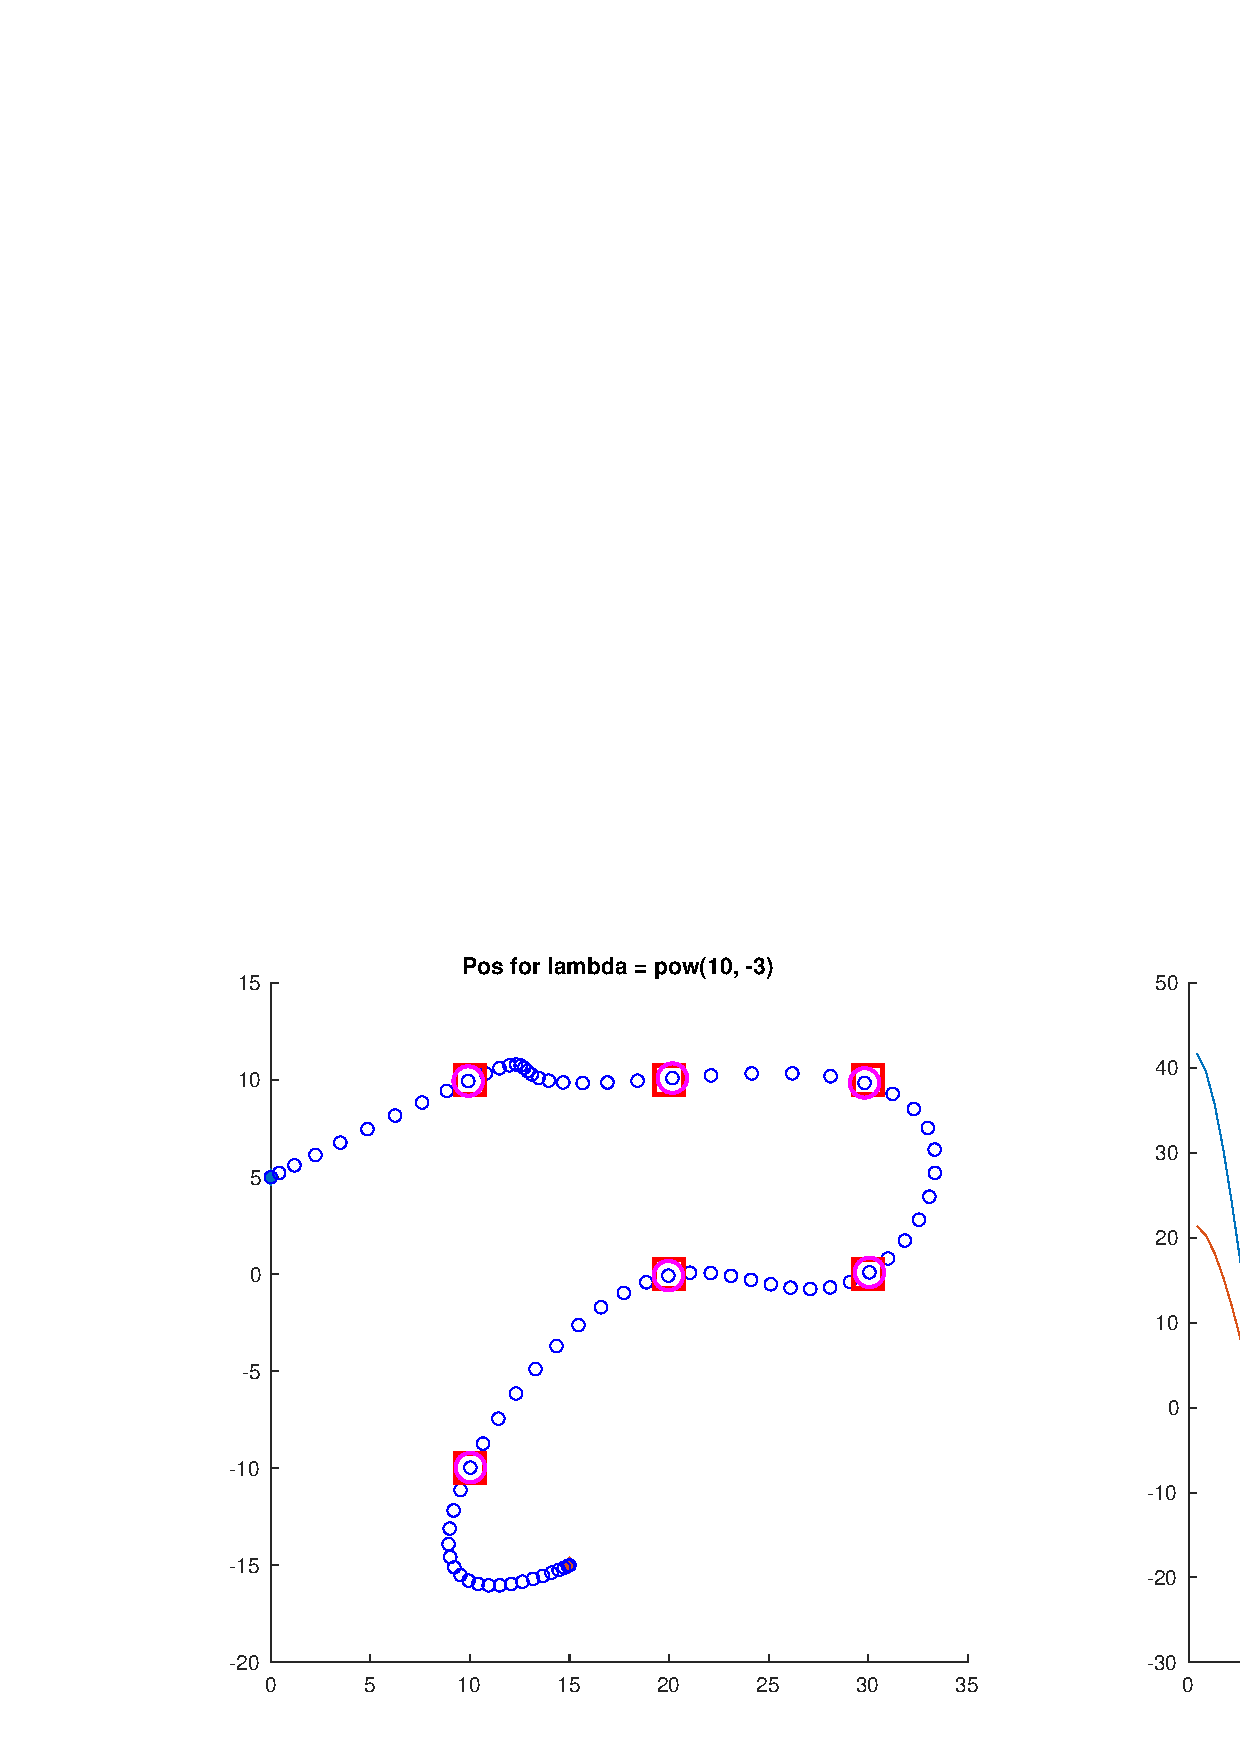
\includegraphics[width=0.5\linewidth]{part1/figures/task1/1_-3.pdf}\hspace{0em}
    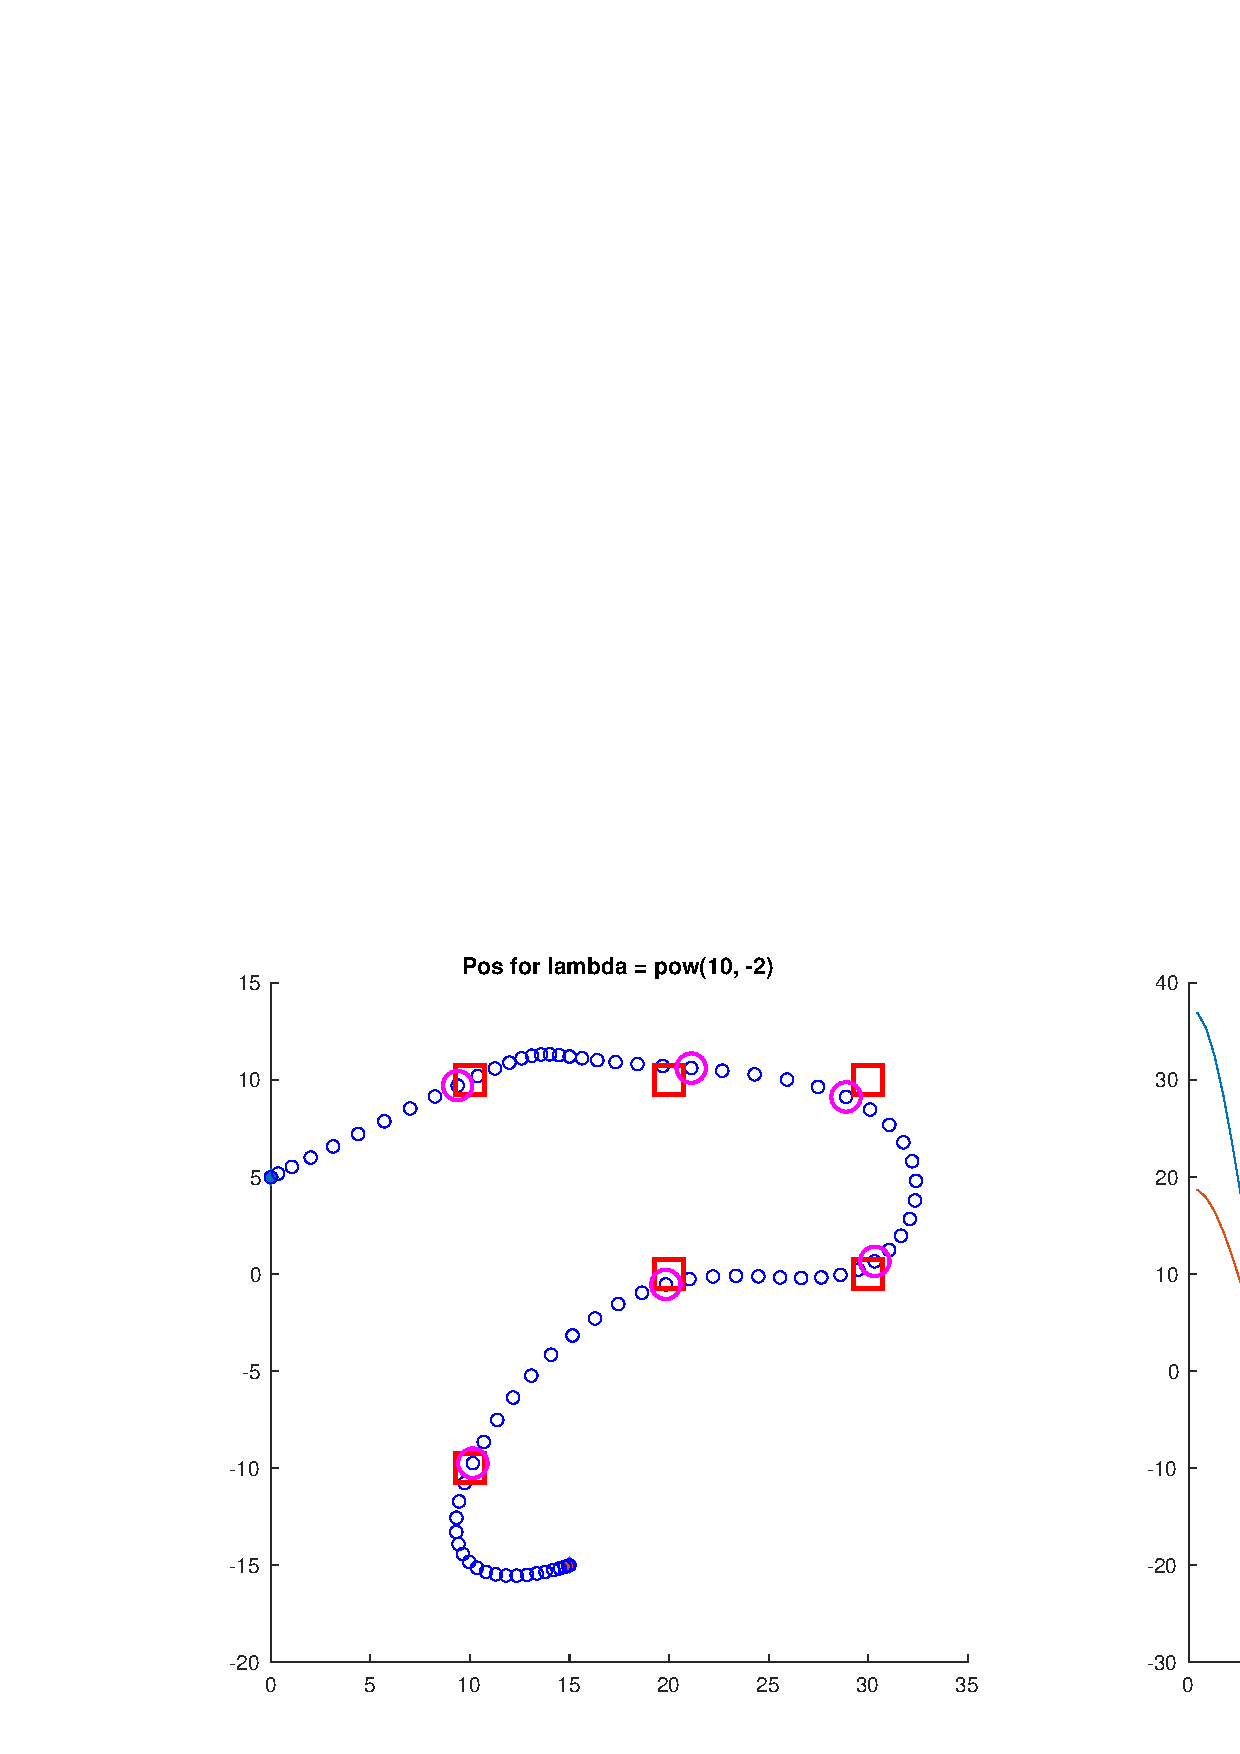
\includegraphics[width=0.5\linewidth]{part1/figures/task1/1_-2.pdf}
\end{subfigure}
\begin{subfigure}
    \centering
    \makebox[\linewidth]{%
        \hspace*{4px}
        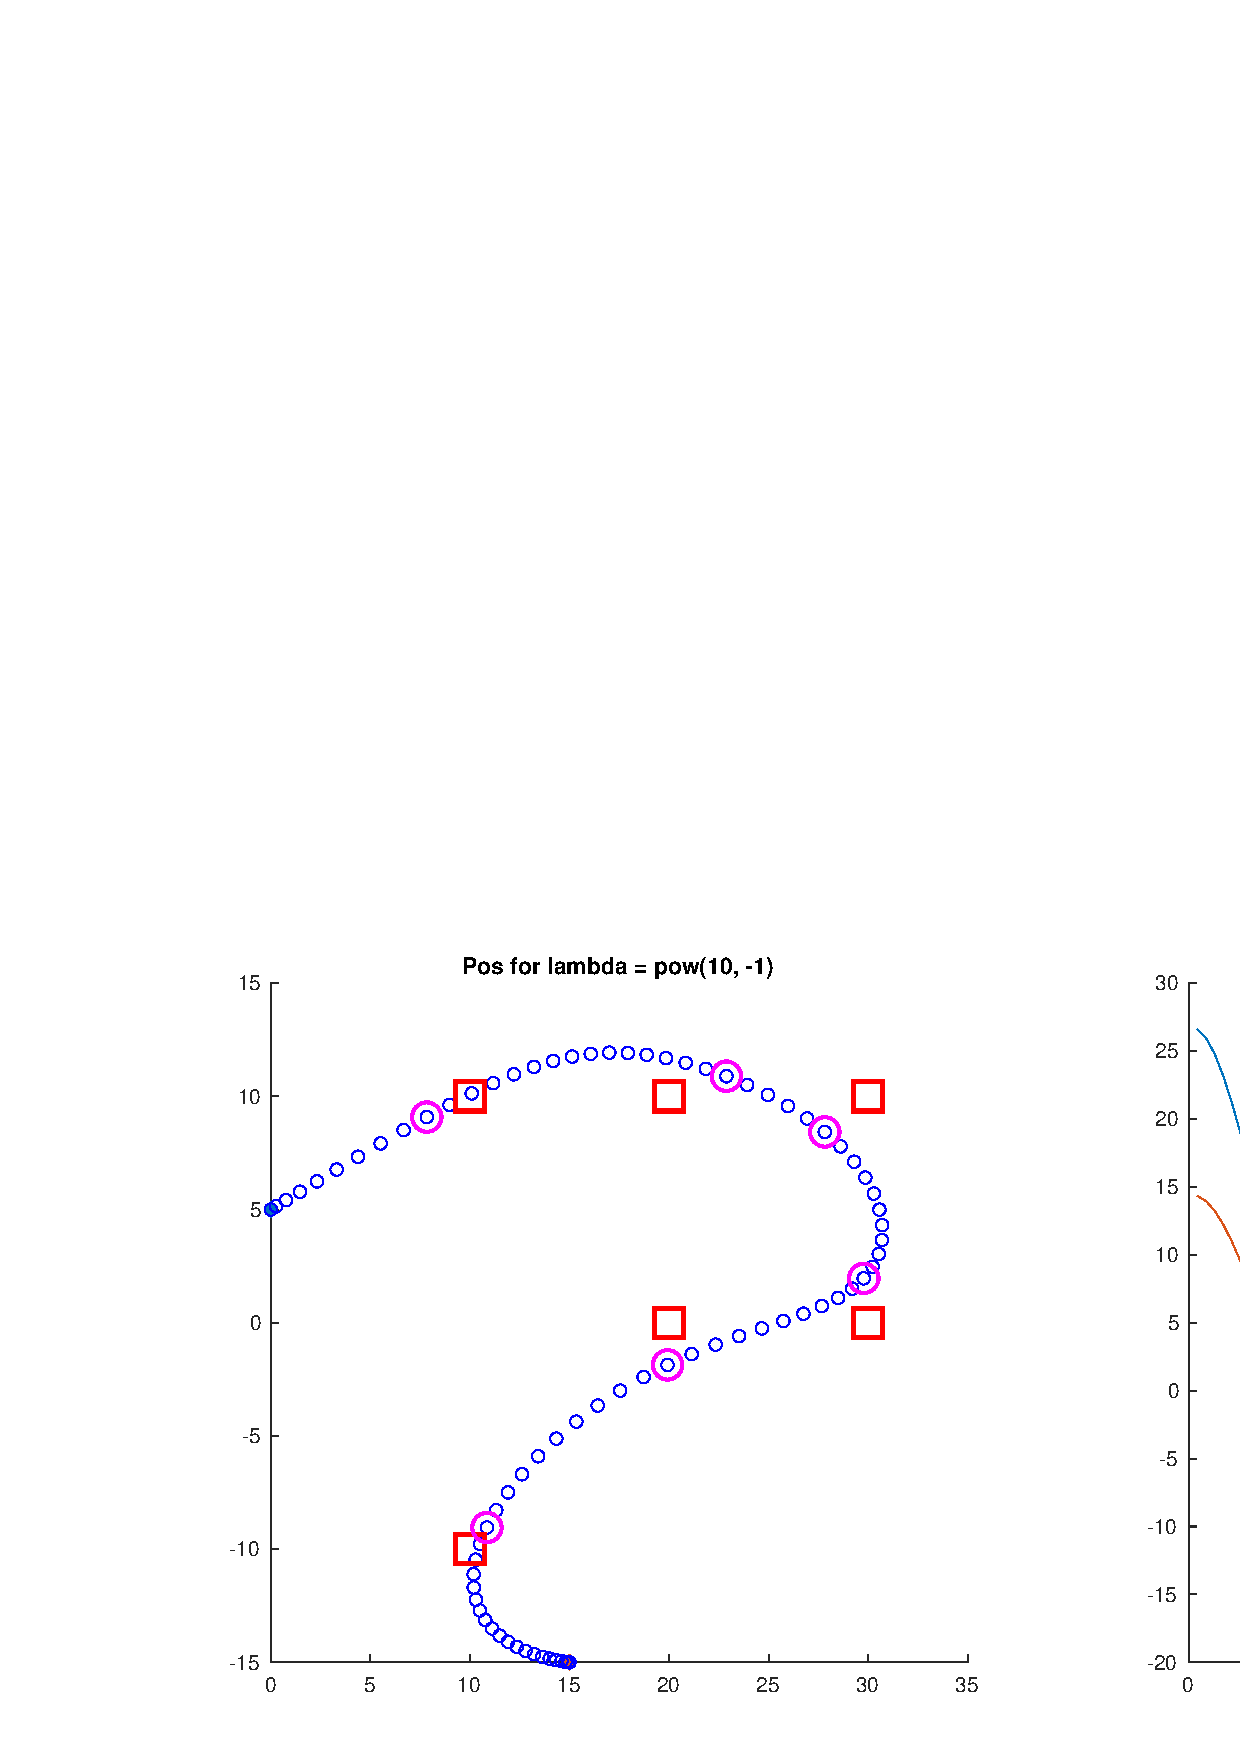
\includegraphics[width=\linewidth + 22px]{part1/figures/task1/1_-1.pdf}
    }
\end{subfigure}
\begin{subfigure}
    \centering
    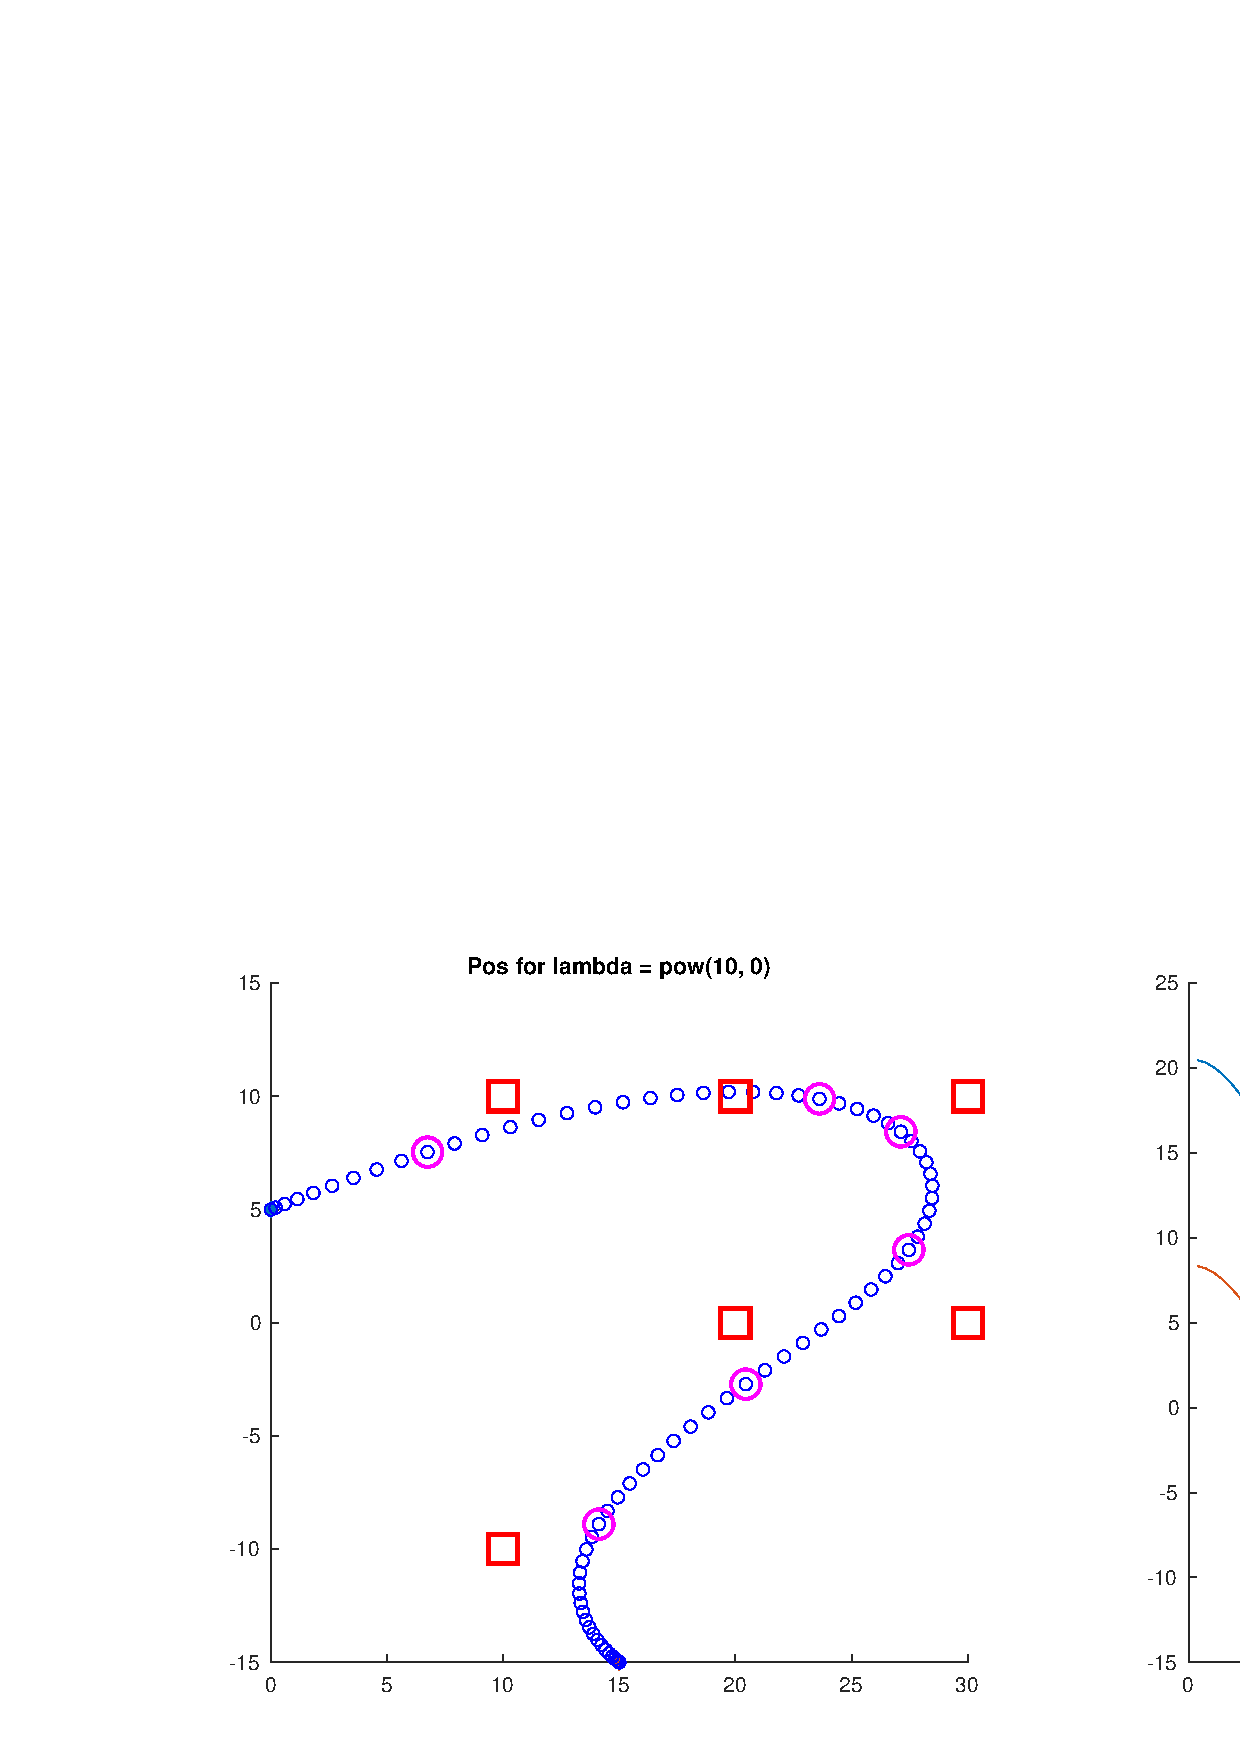
\includegraphics[width=0.5\linewidth]{part1/figures/task1/1_0.pdf}\hspace{0em}
    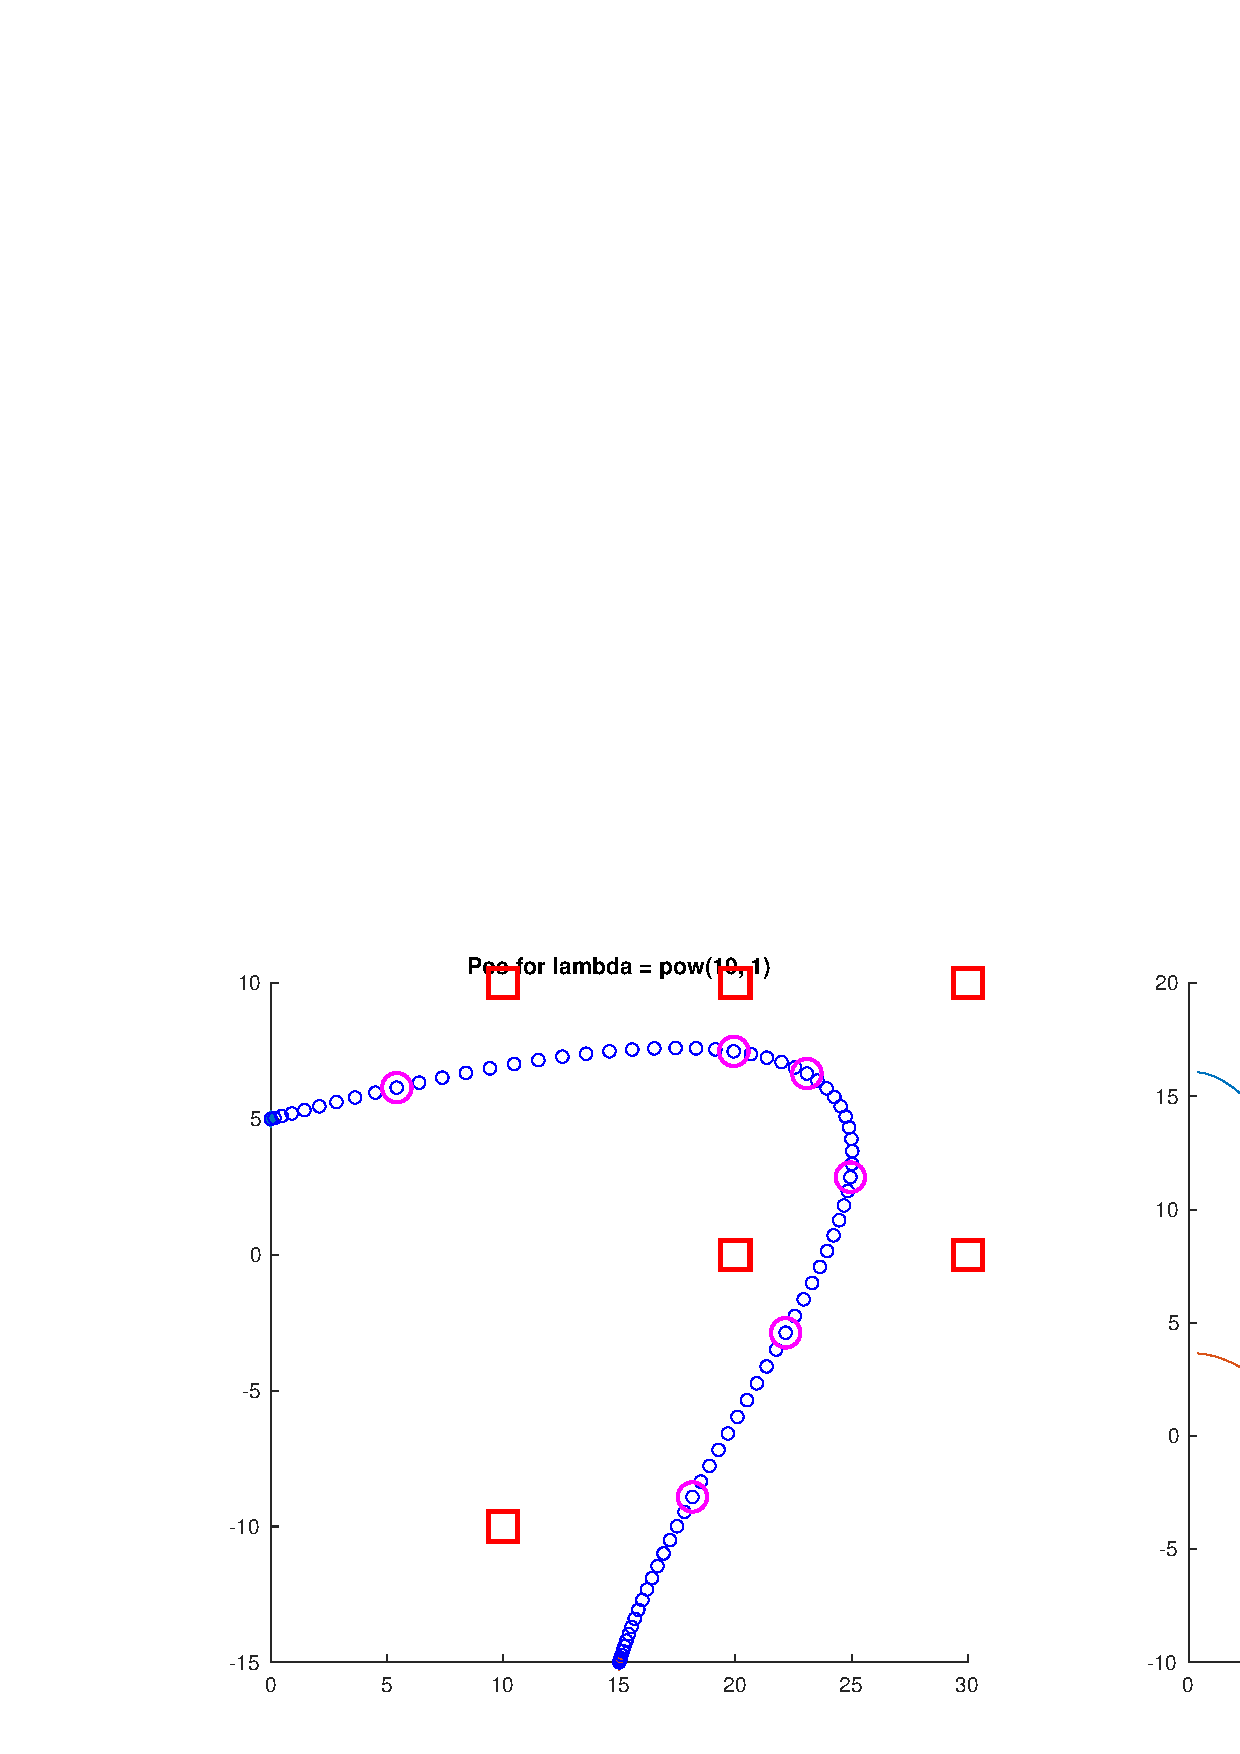
\includegraphics[width=0.5\linewidth]{part1/figures/task1/1_1.pdf}
\end{subfigure}
\begin{subfigure}
    \centering
    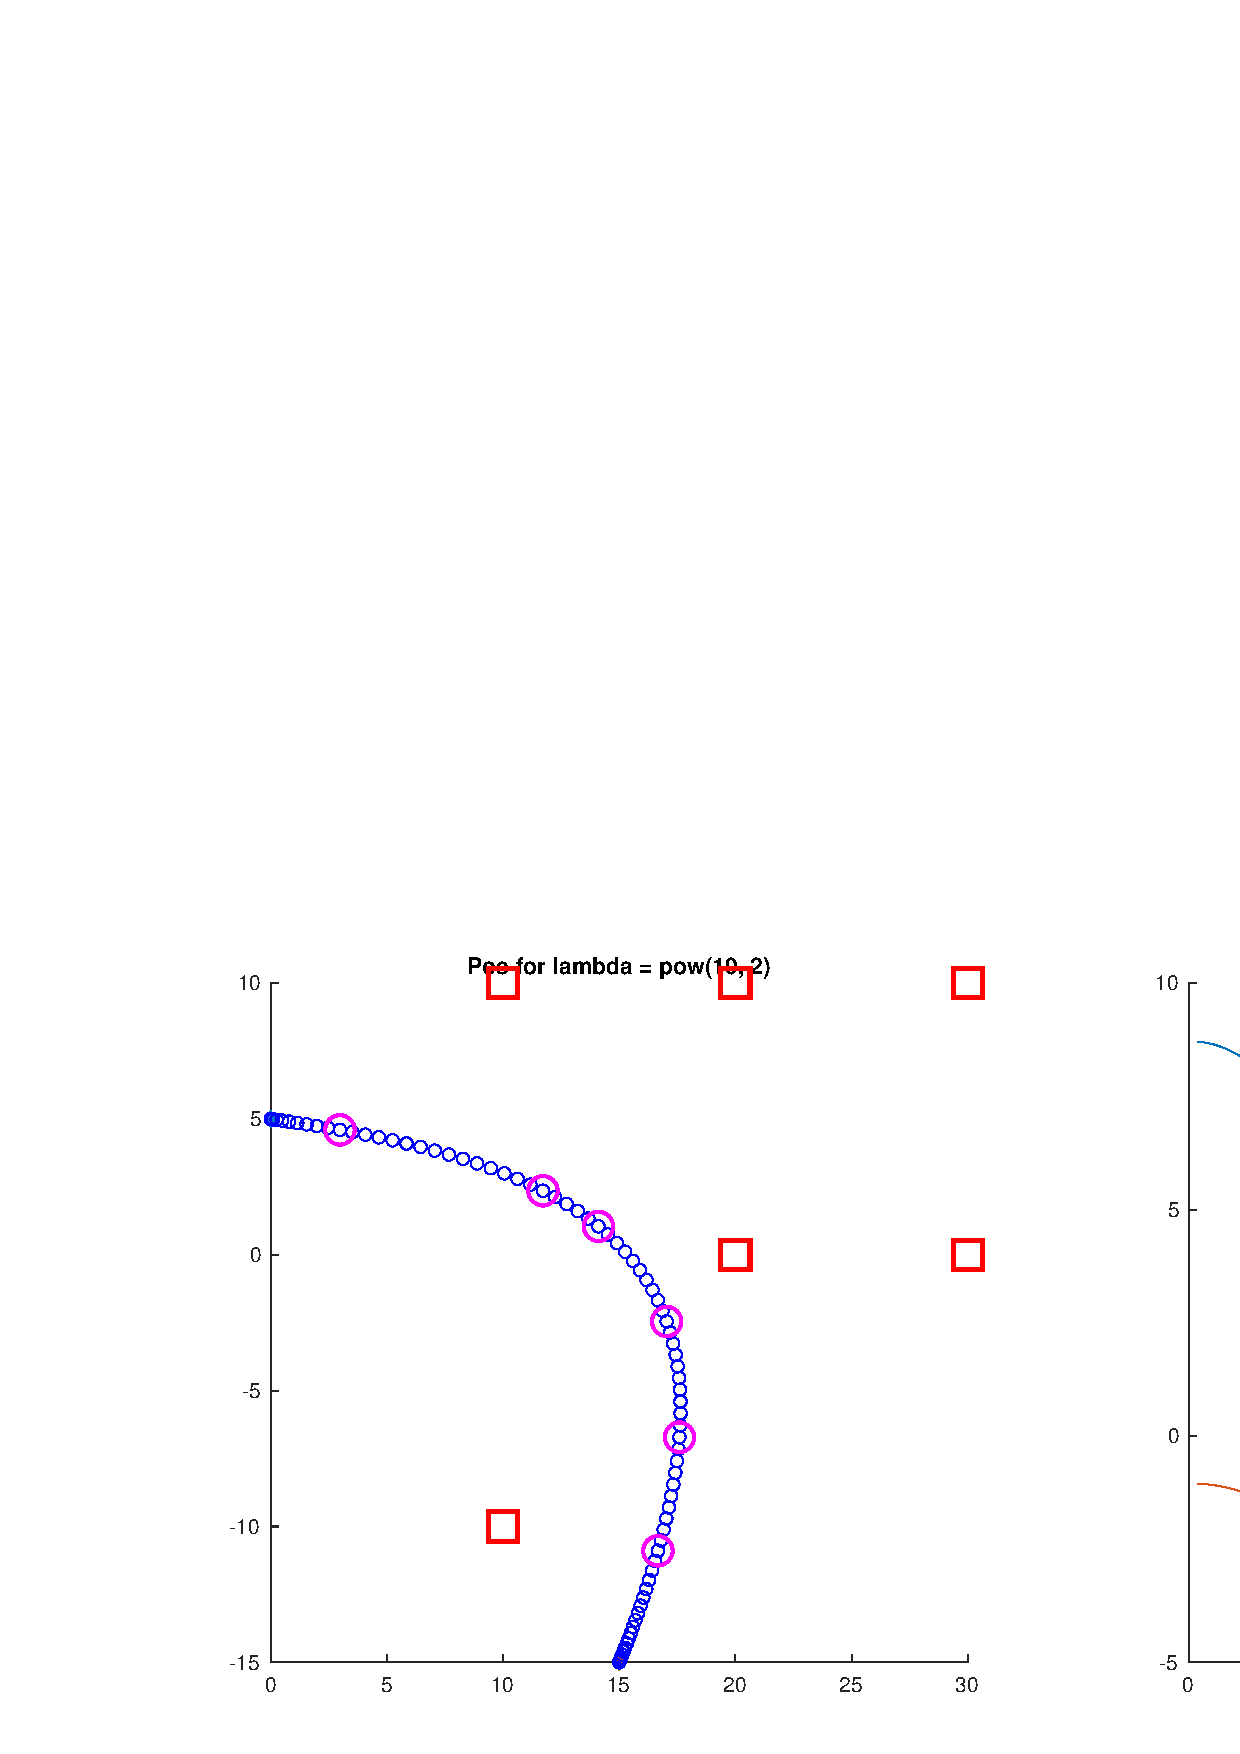
\includegraphics[width=0.5\linewidth]{part1/figures/task1/1_2.pdf}\hspace{0em}
    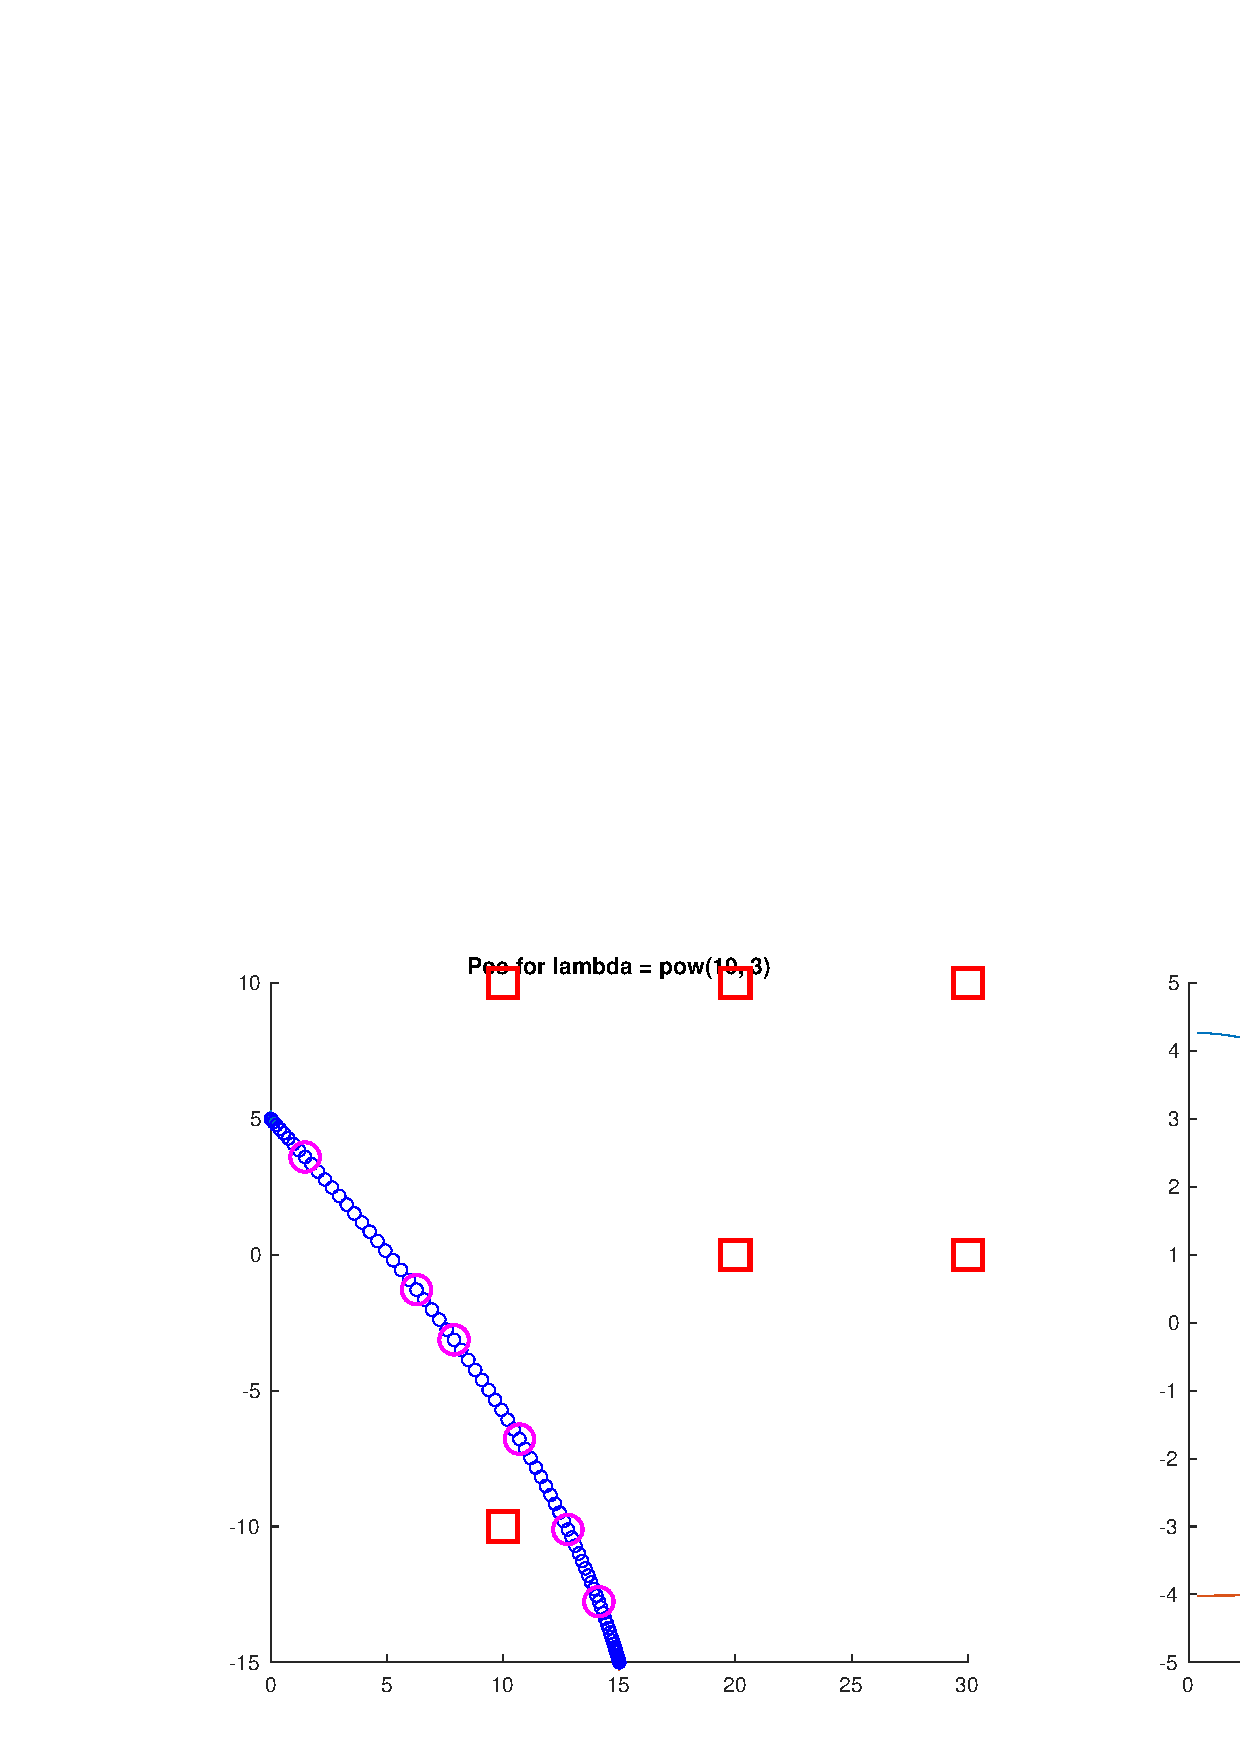
\includegraphics[width=0.5\linewidth]{part1/figures/task1/1_3.pdf}
\end{subfigure}
\caption{Robot positions and control signal for Task 1.}
\label{fig:task1:graphs}
\end{figure}

\clearpage
\subsection{Task 2}
%\noindent\fcolorbox{black}{lightgray}{
%    \parbox{\textwidth}{ \textbf{Task 2.} Redo task 1 for the optimization problem~\eqref{prob2}. 
%    }
%}
Code utilized in the task 2 is same as in Task 1, except for the objective function, which is defined as described in Listing \ref{task2:code:objective}. The results are described in the Table \ref{task2:table:results}. The robot positions and control signal are visualized in the Figure \ref{fig:task2:graphs}.

\begin{lstlisting}[label=task2:code:objective, caption=Objective function used in Task 2., float=!htb]
minimize(sum(vec_sqr_sum(E*x(:,tau+1) - w))...
    + lambda*sum(norms(delta, 2)));
\end{lstlisting}

\begin{figure}[!htb]
\begin{subfigure}
    \centering
    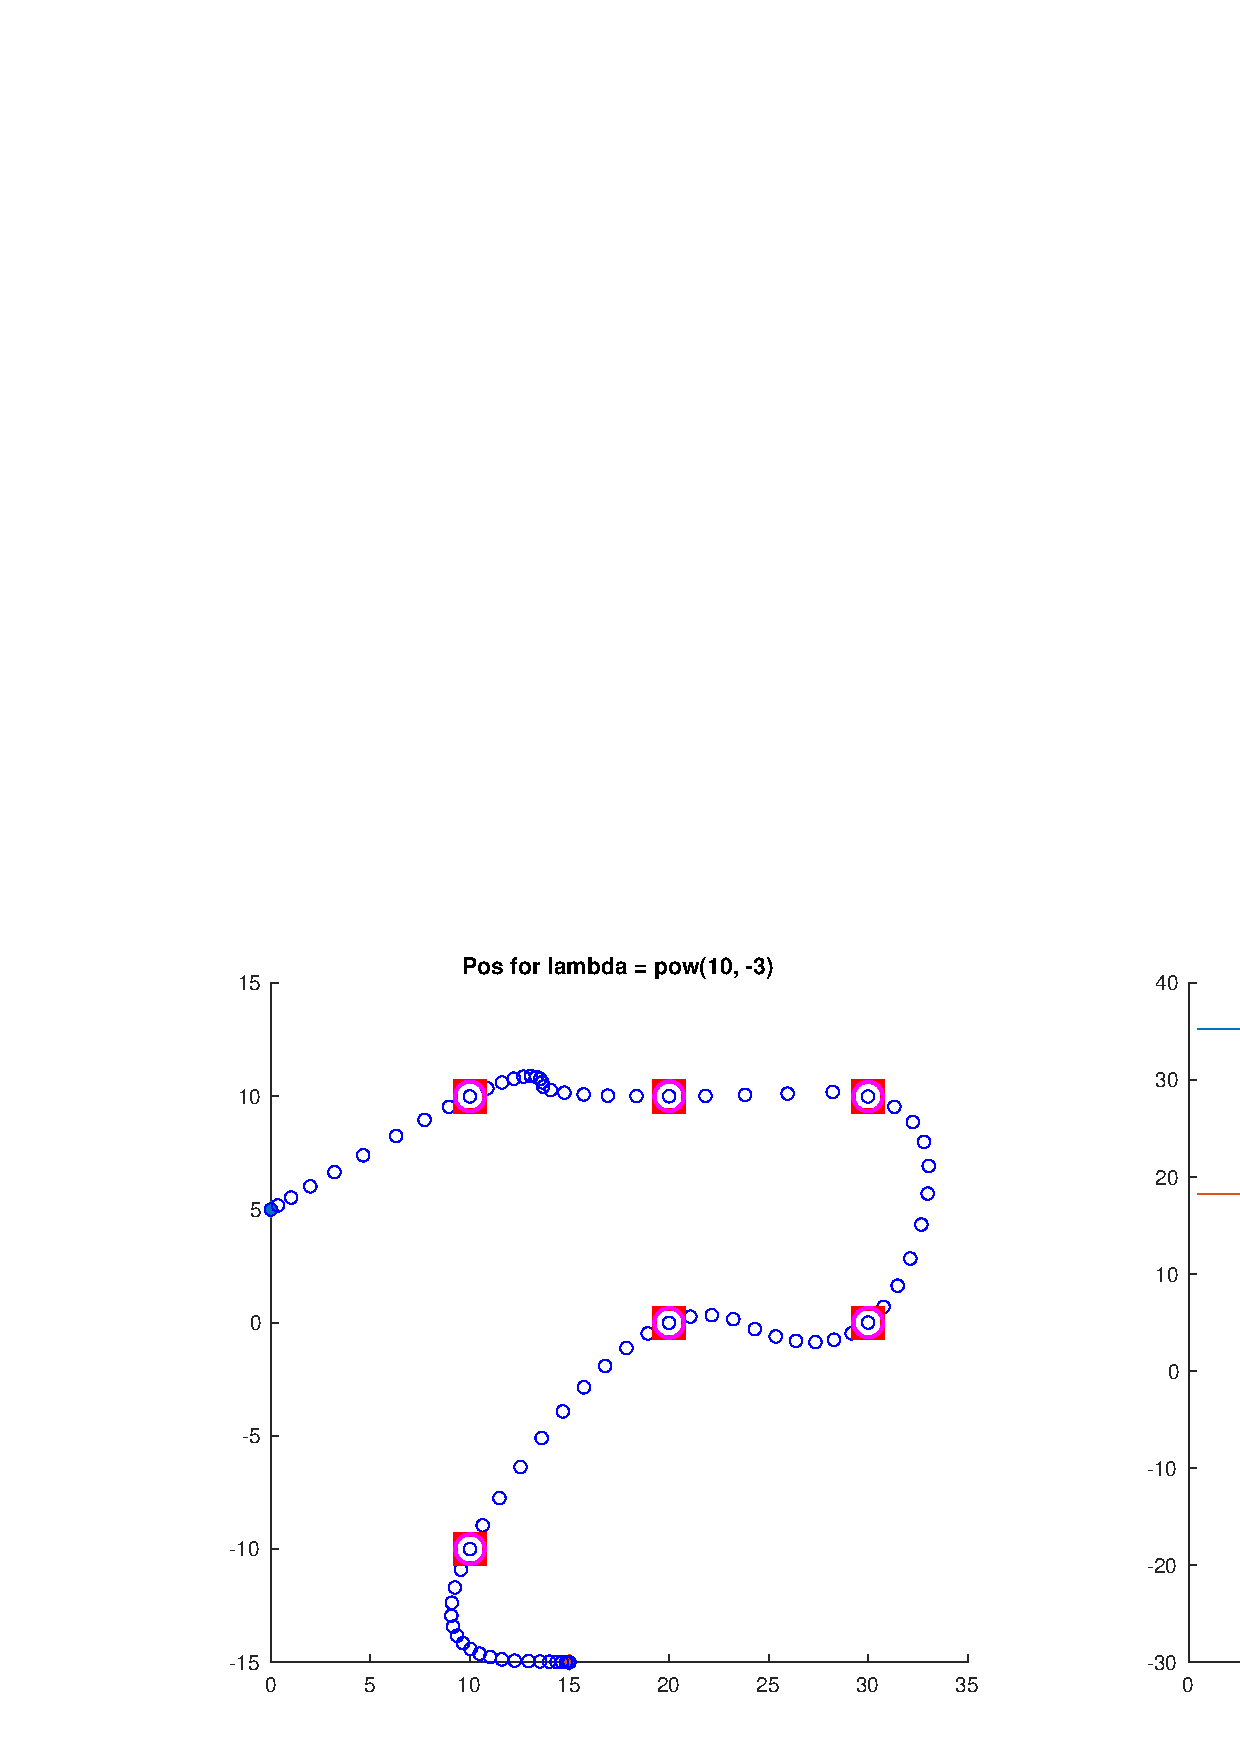
\includegraphics[width=0.5\linewidth]{part1/figures/task2/2_-3.pdf}\hspace{0em}
    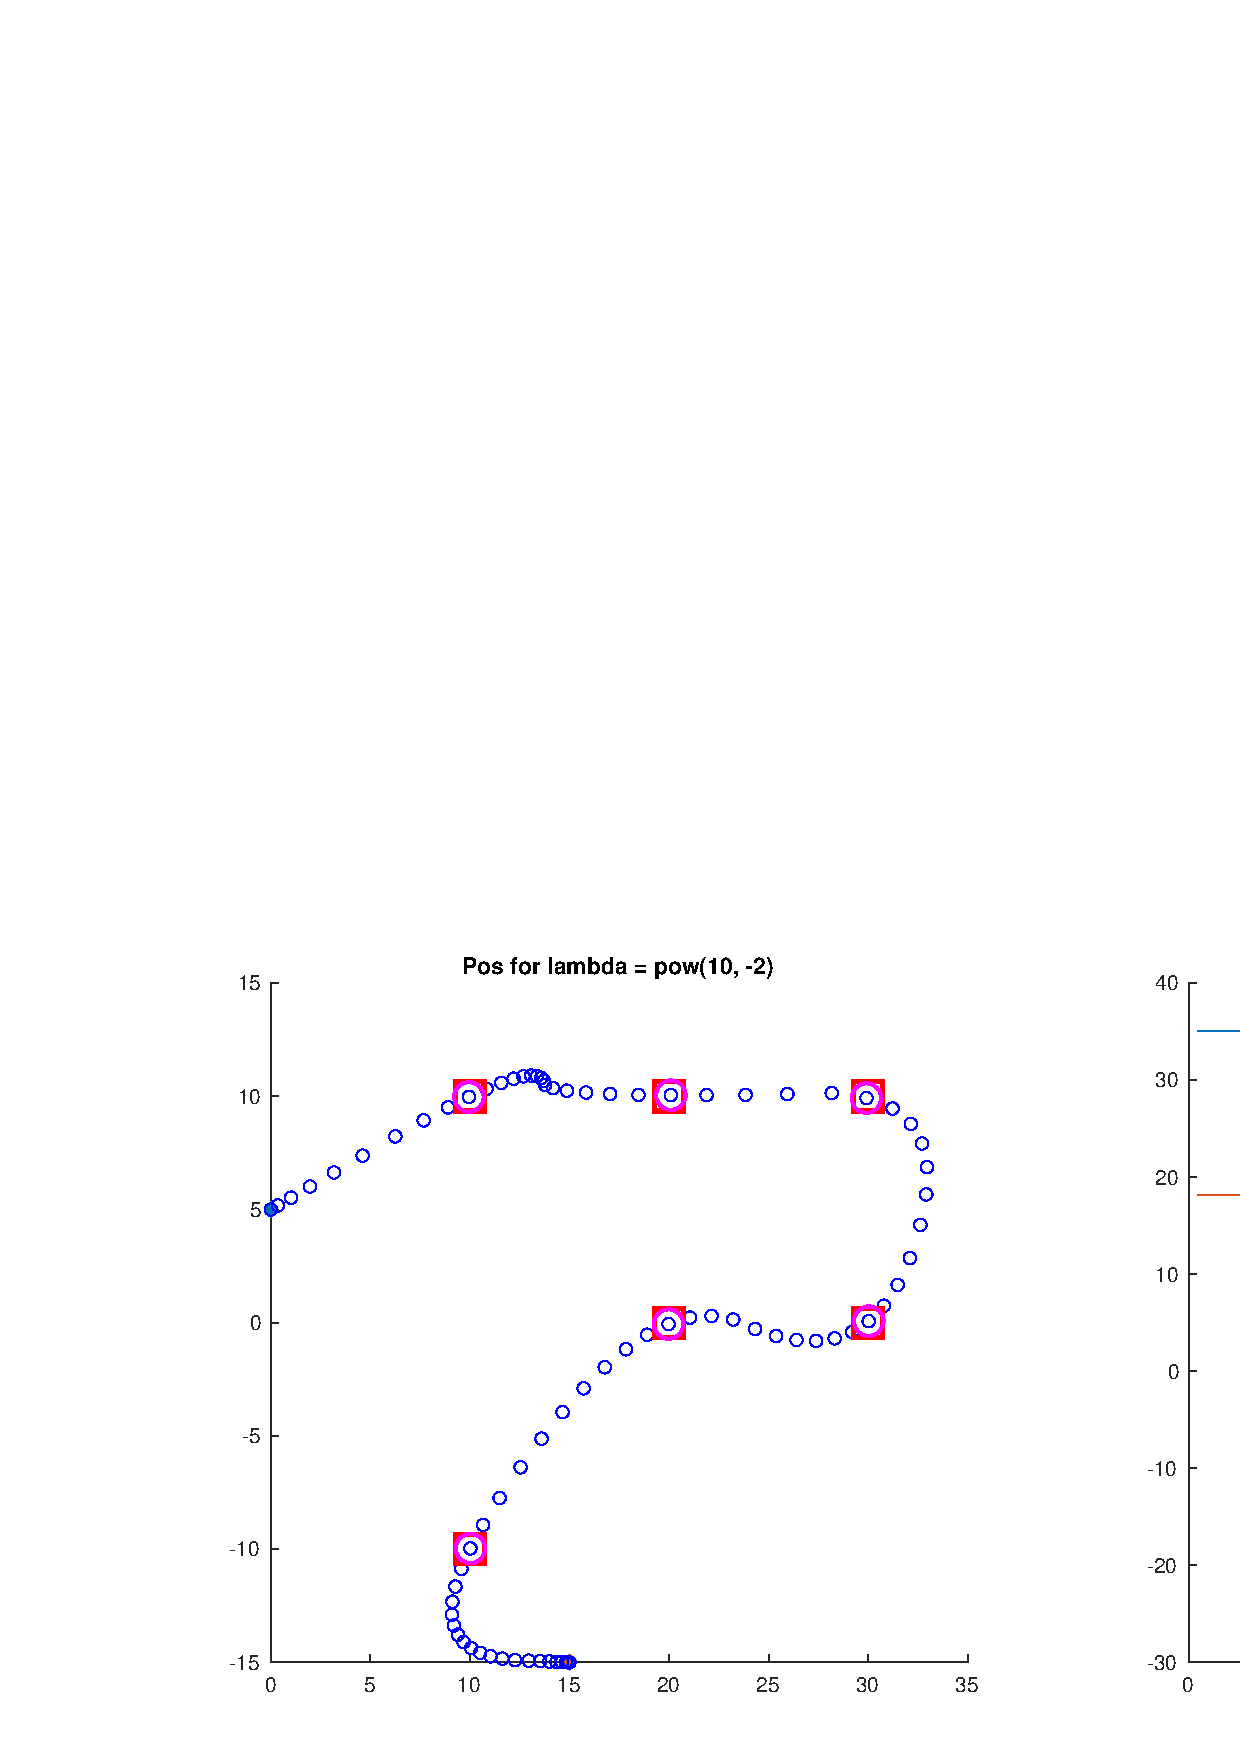
\includegraphics[width=0.5\linewidth]{part1/figures/task2/2_-2.pdf}
\end{subfigure}
\begin{subfigure}
    \centering
    \makebox[\linewidth]{%
        \hspace*{4px}
        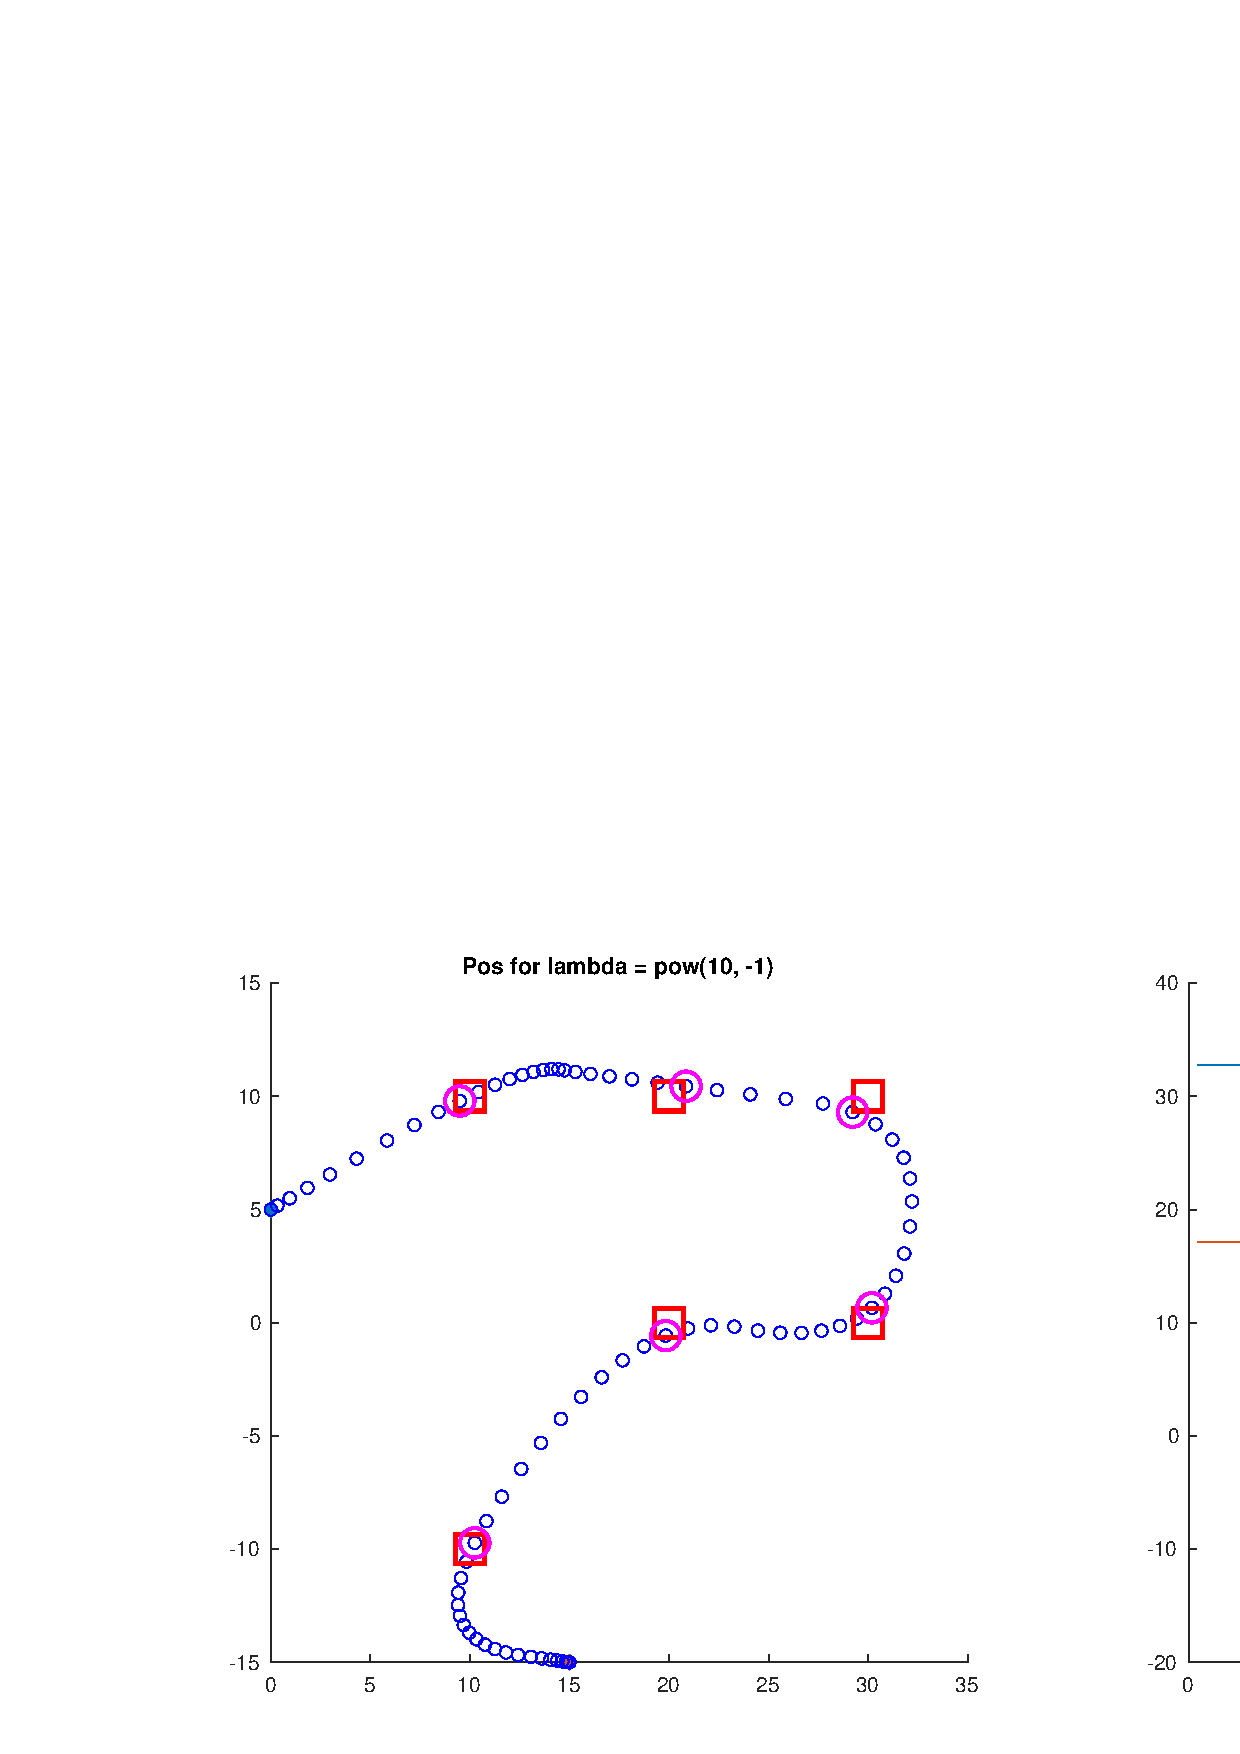
\includegraphics[width=\linewidth + 22px]{part1/figures/task2/2_-1.pdf}
    }
\end{subfigure}
\begin{subfigure}
    \centering
    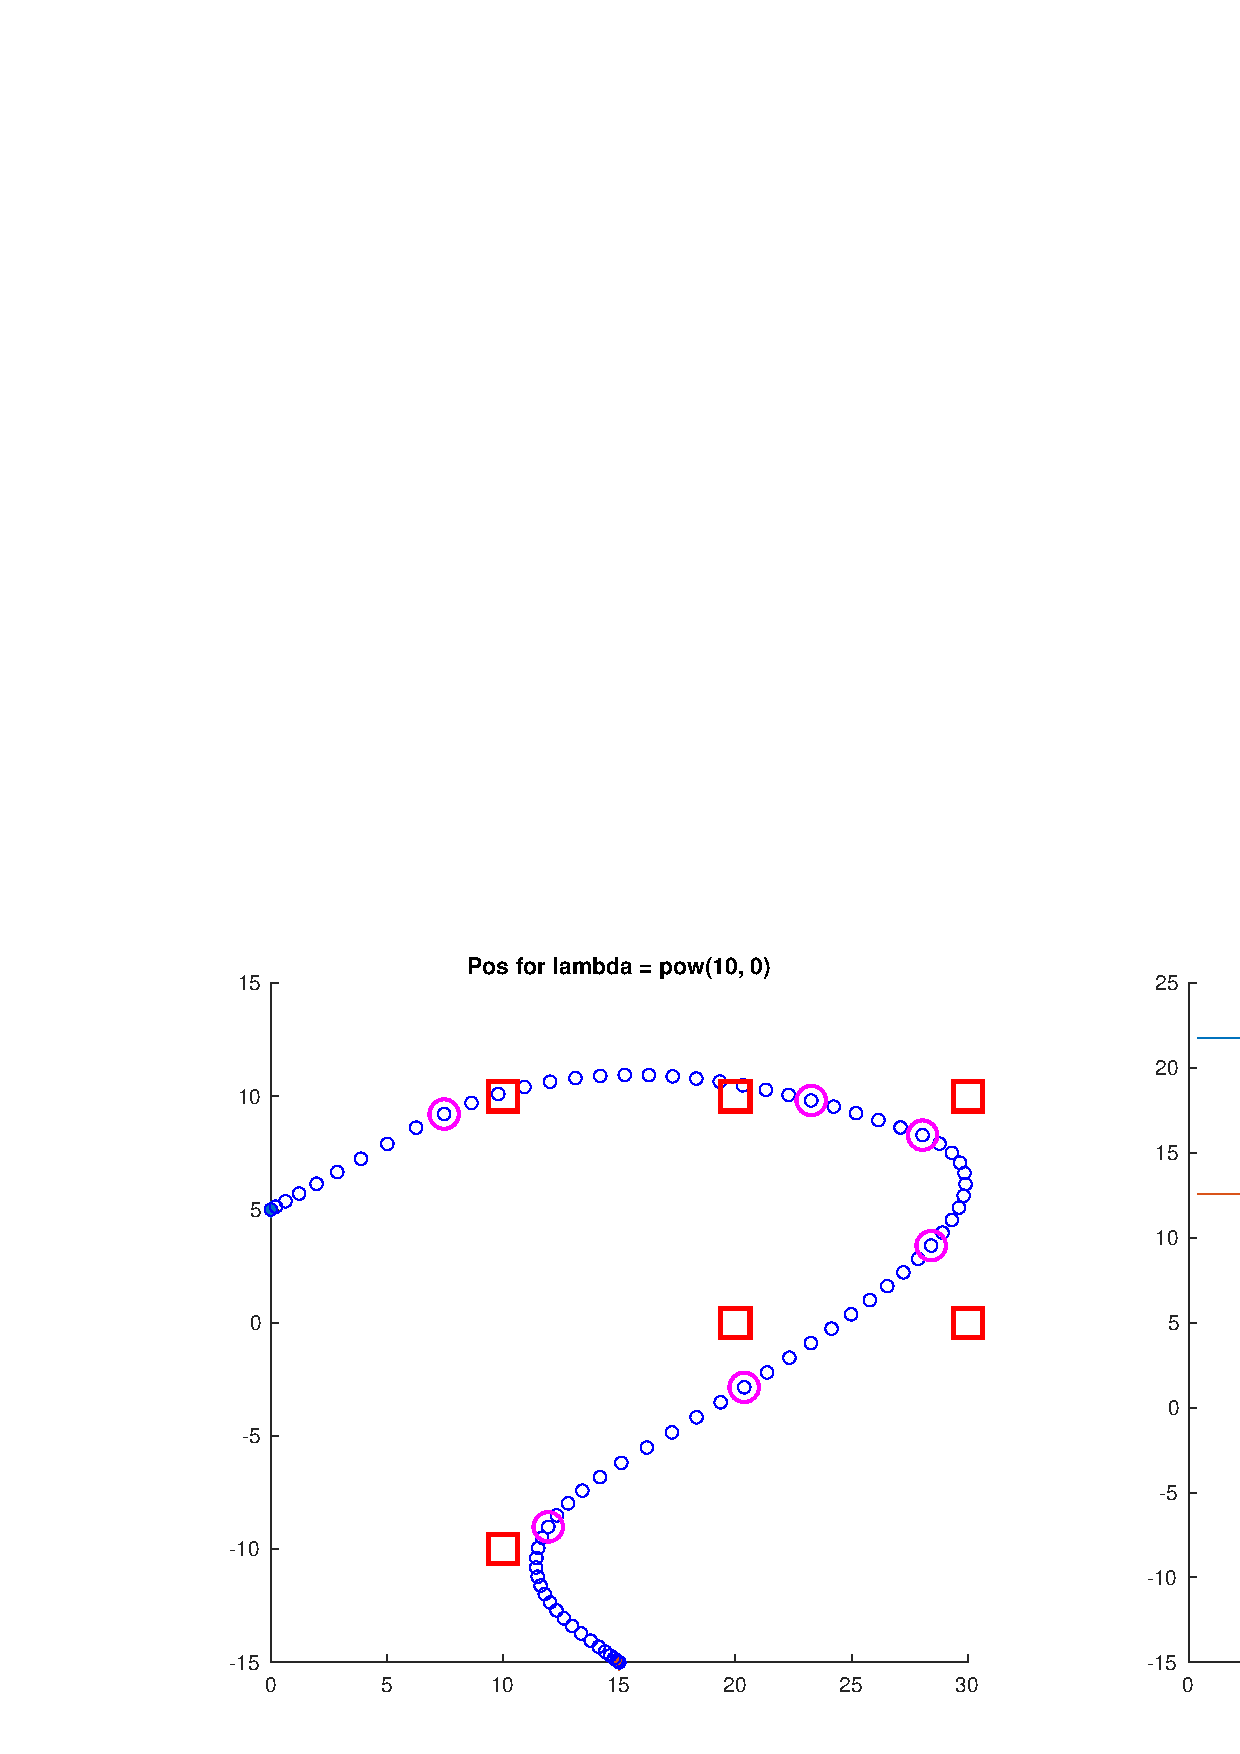
\includegraphics[width=0.5\linewidth]{part1/figures/task2/2_0.pdf}\hspace{0em}
    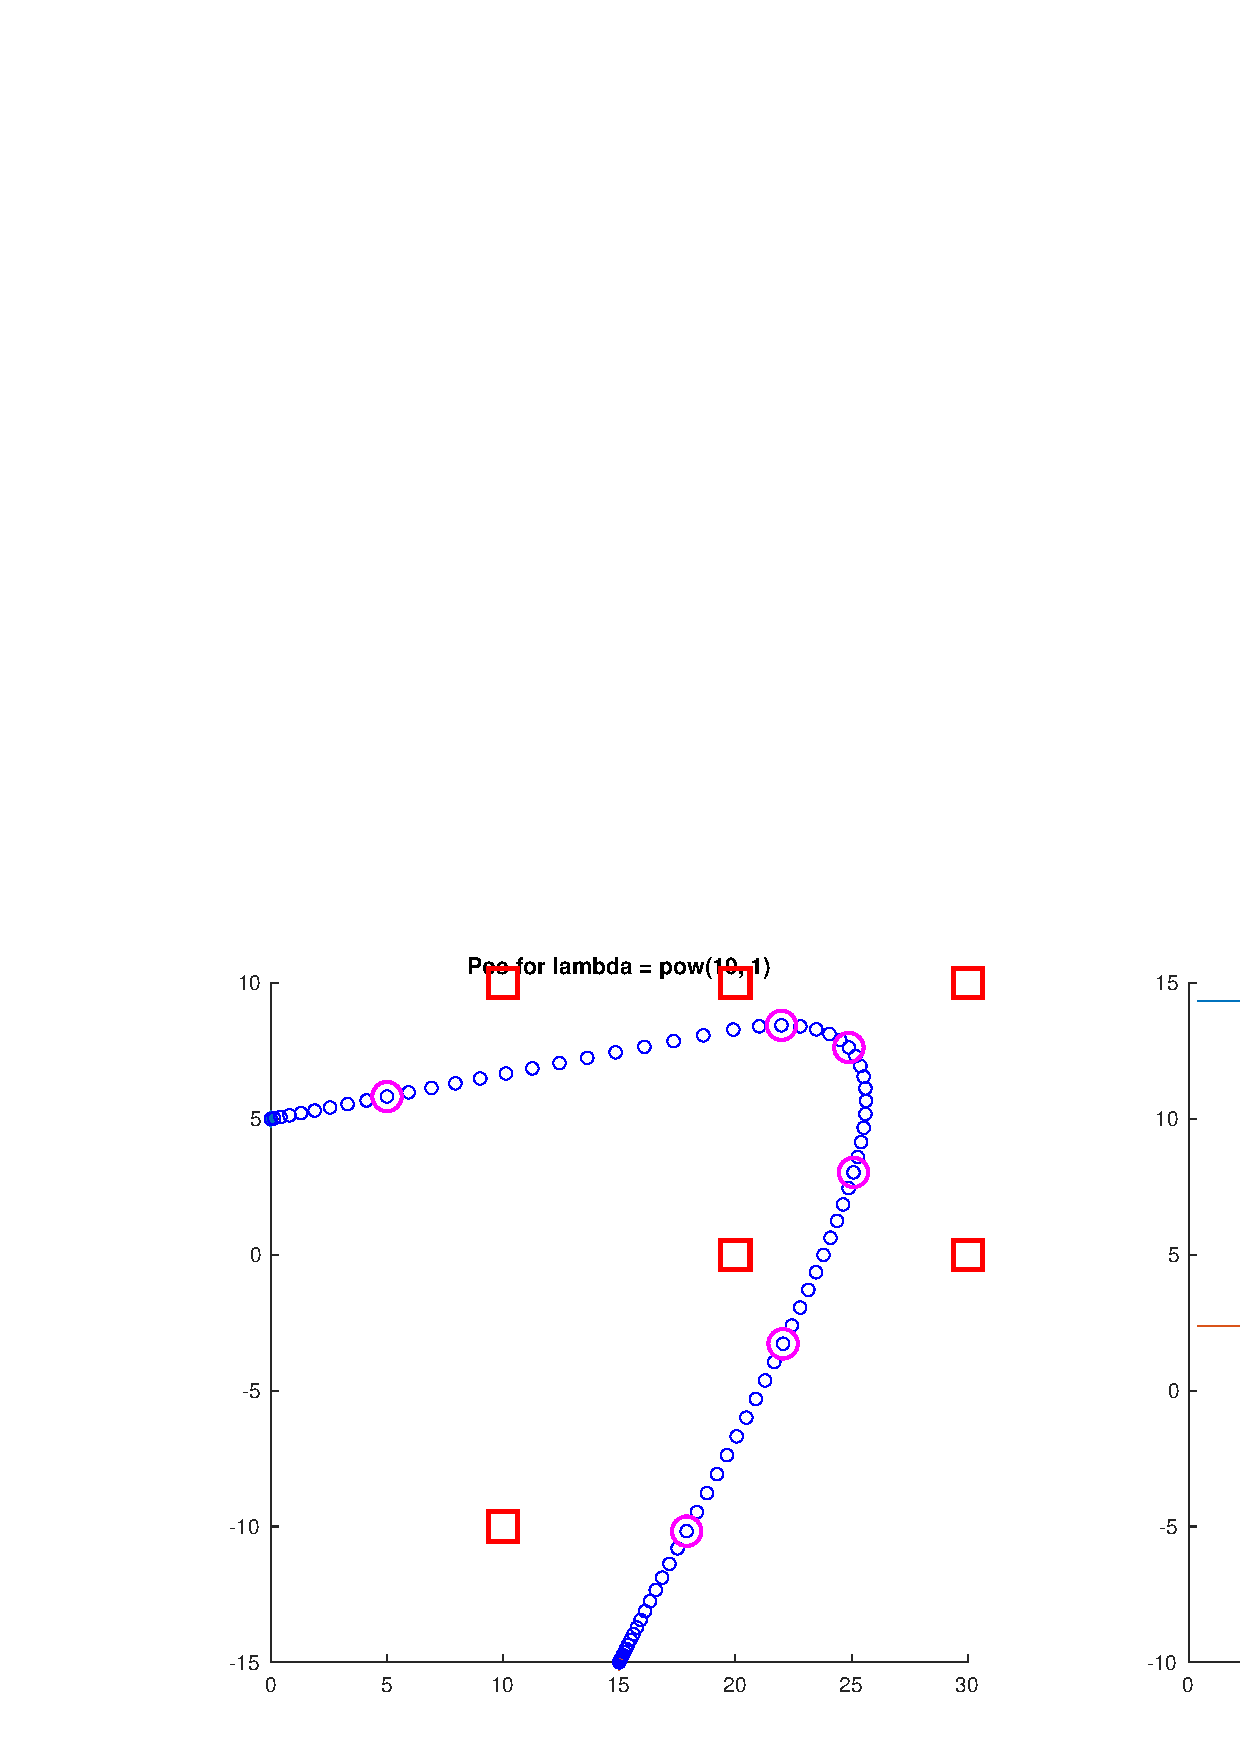
\includegraphics[width=0.5\linewidth]{part1/figures/task2/2_1.pdf}
\end{subfigure}
\begin{subfigure}
    \centering
    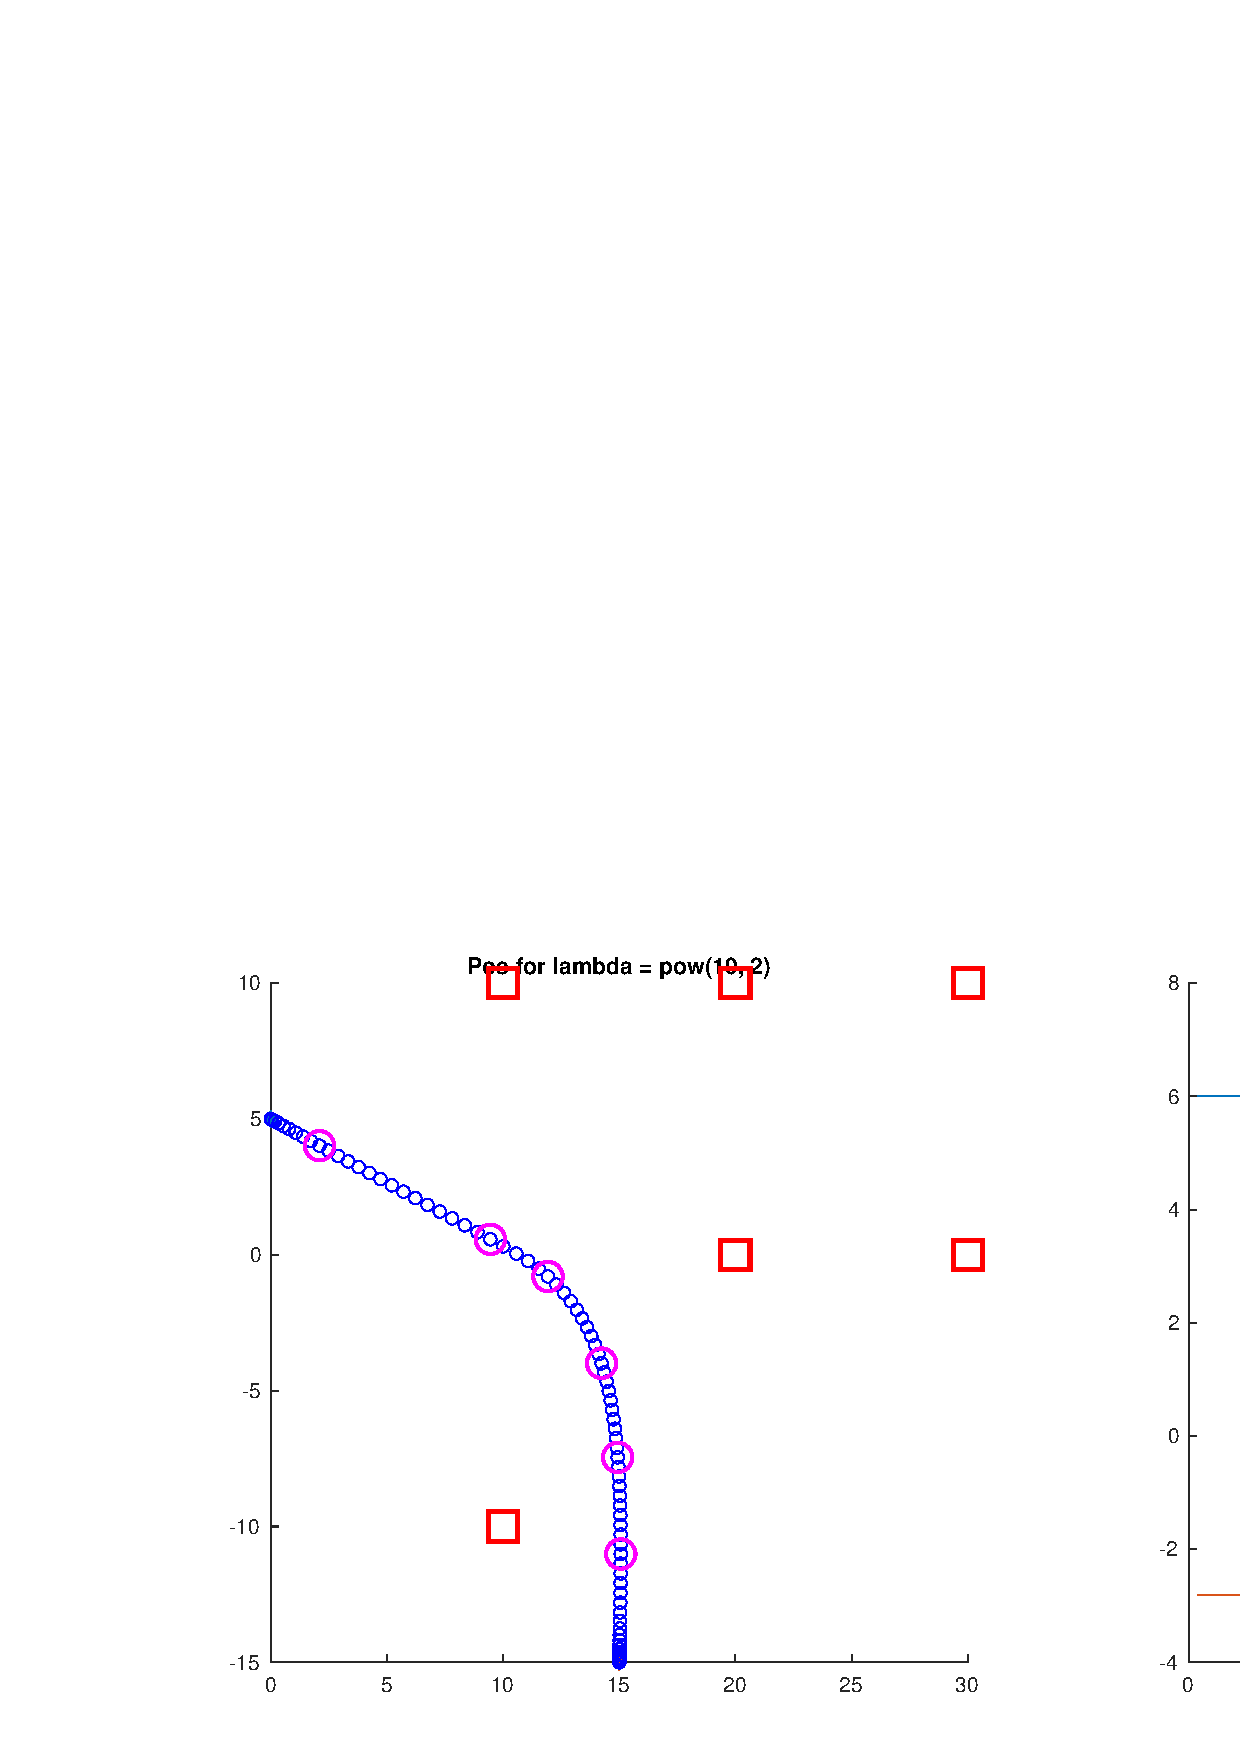
\includegraphics[width=0.5\linewidth]{part1/figures/task2/2_2.pdf}\hspace{0em}
    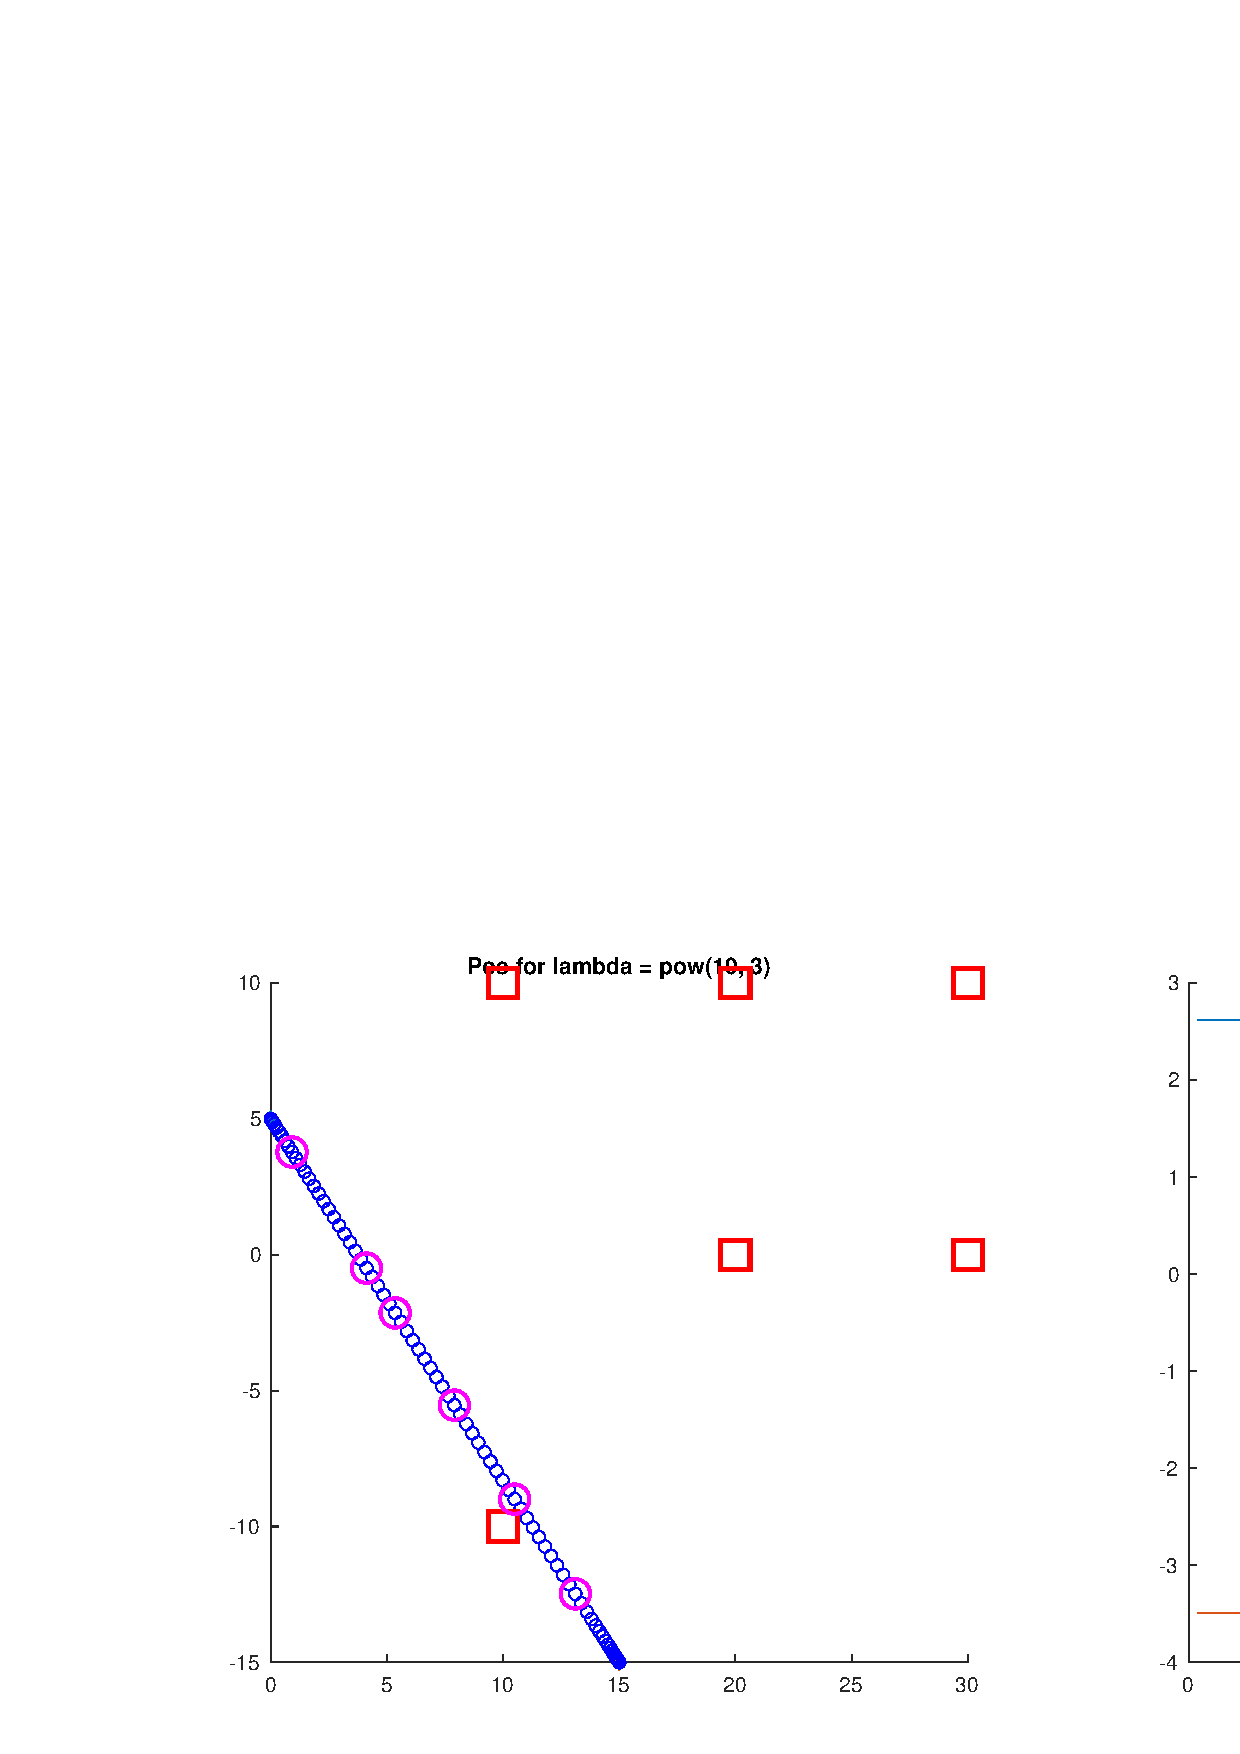
\includegraphics[width=0.5\linewidth]{part1/figures/task2/2_3.pdf}
\end{subfigure}
\caption{Robot positions and control signal for Task 2.}
\label{fig:task2:graphs}
\end{figure}

\subsection{Task 3}
%\noindent\fcolorbox{black}{lightgray}{
%    \parbox{\textwidth}{ \textbf{Task 3.} Redo task 1 for the optimization problem~\eqref{prob3}. 
% }}

\begin{lstlisting}[caption=Objective function used in Task 3., label=task3:code:objective, float=!htb]
minimize(sum(vec_sqr_sum(E*x(:,tau+1) - w)...
                ) + lambda*sum(norms(delta, 1)));
\end{lstlisting}

Code utilized in the task 3 is same as in Task 1, except for the objective function, which is defined as described in Listing \ref{task3:code:objective}. The results are described in the Table \ref{task3:table:results}. The robot positions and control signal are visualized in the Figure \ref{fig:task3:graphs}.

\begin{figure}[!htb]
\begin{subfigure}
    \centering
    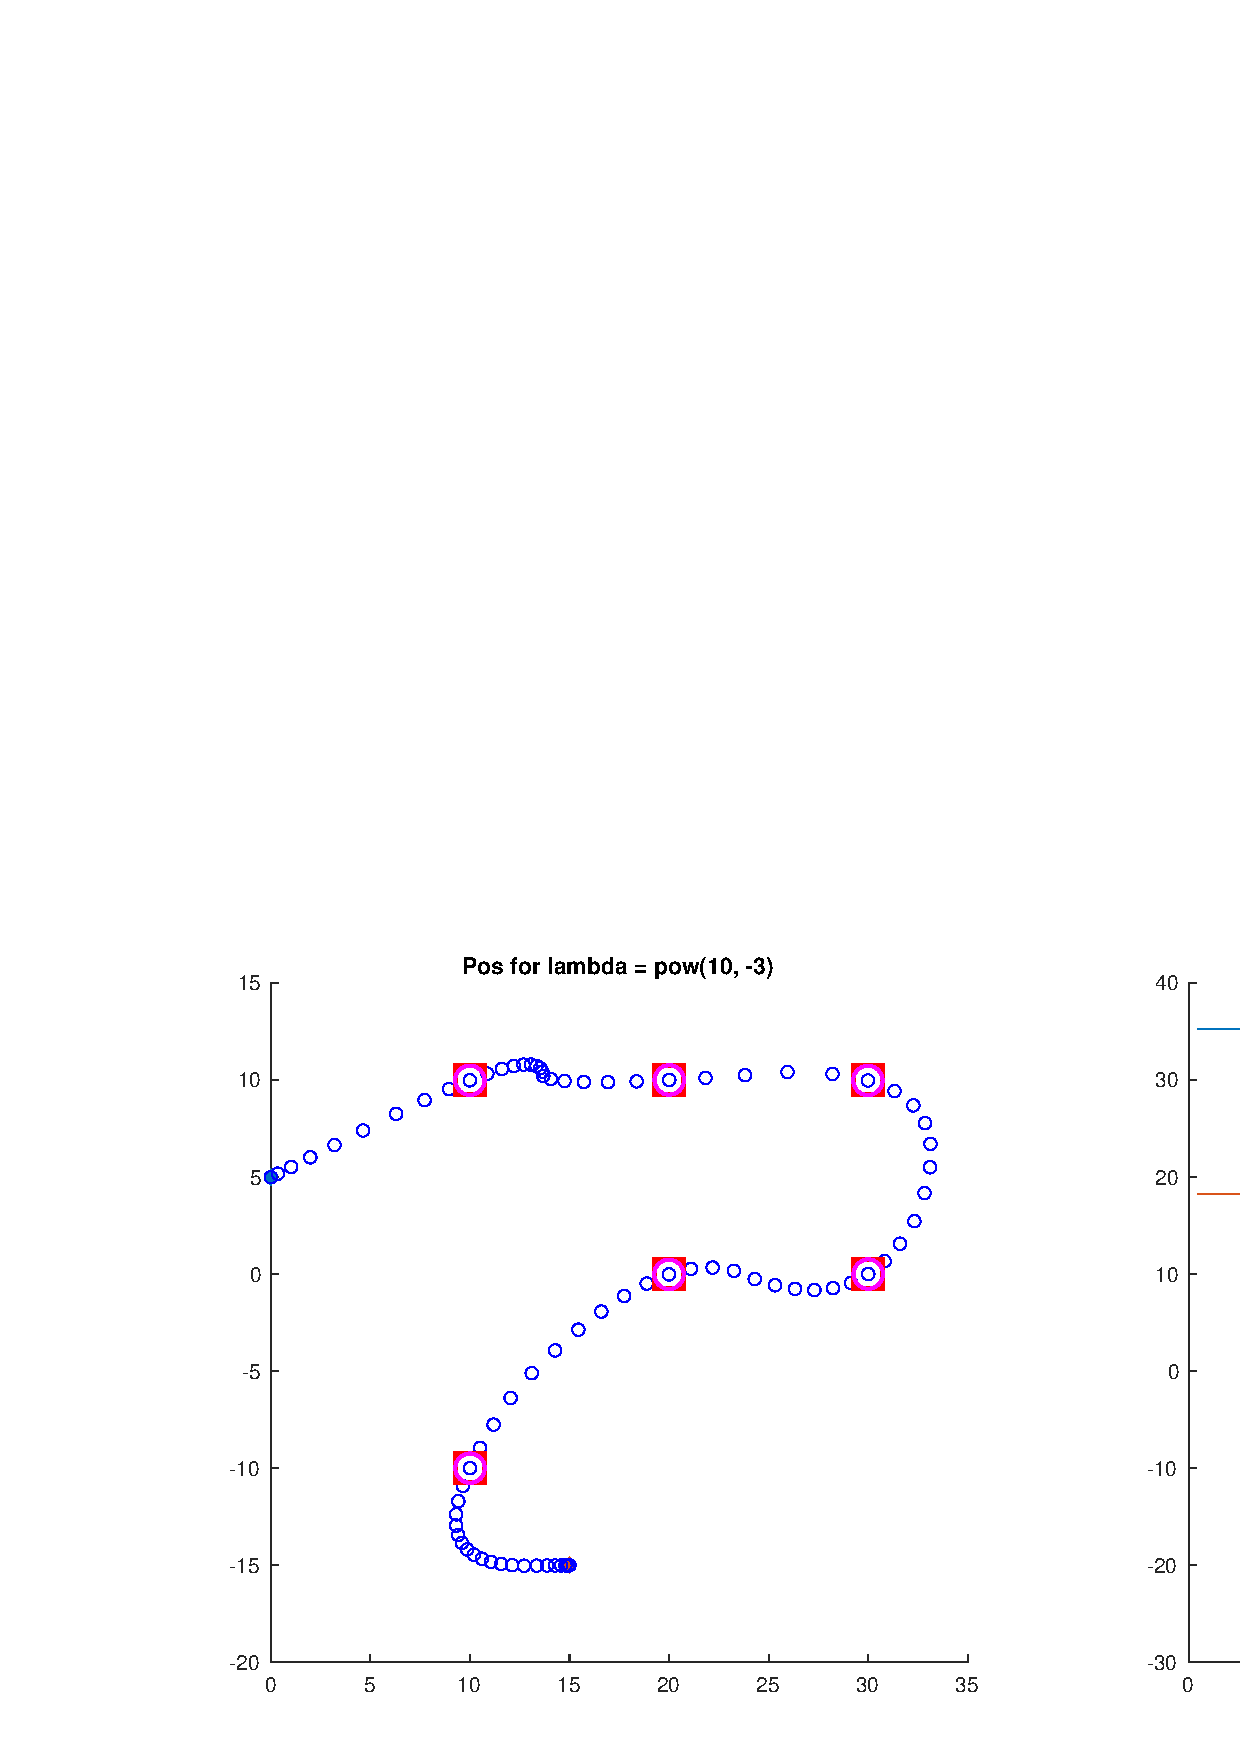
\includegraphics[width=0.5\linewidth]{part1/figures/task3/3_-3.pdf}\hspace{0em}
    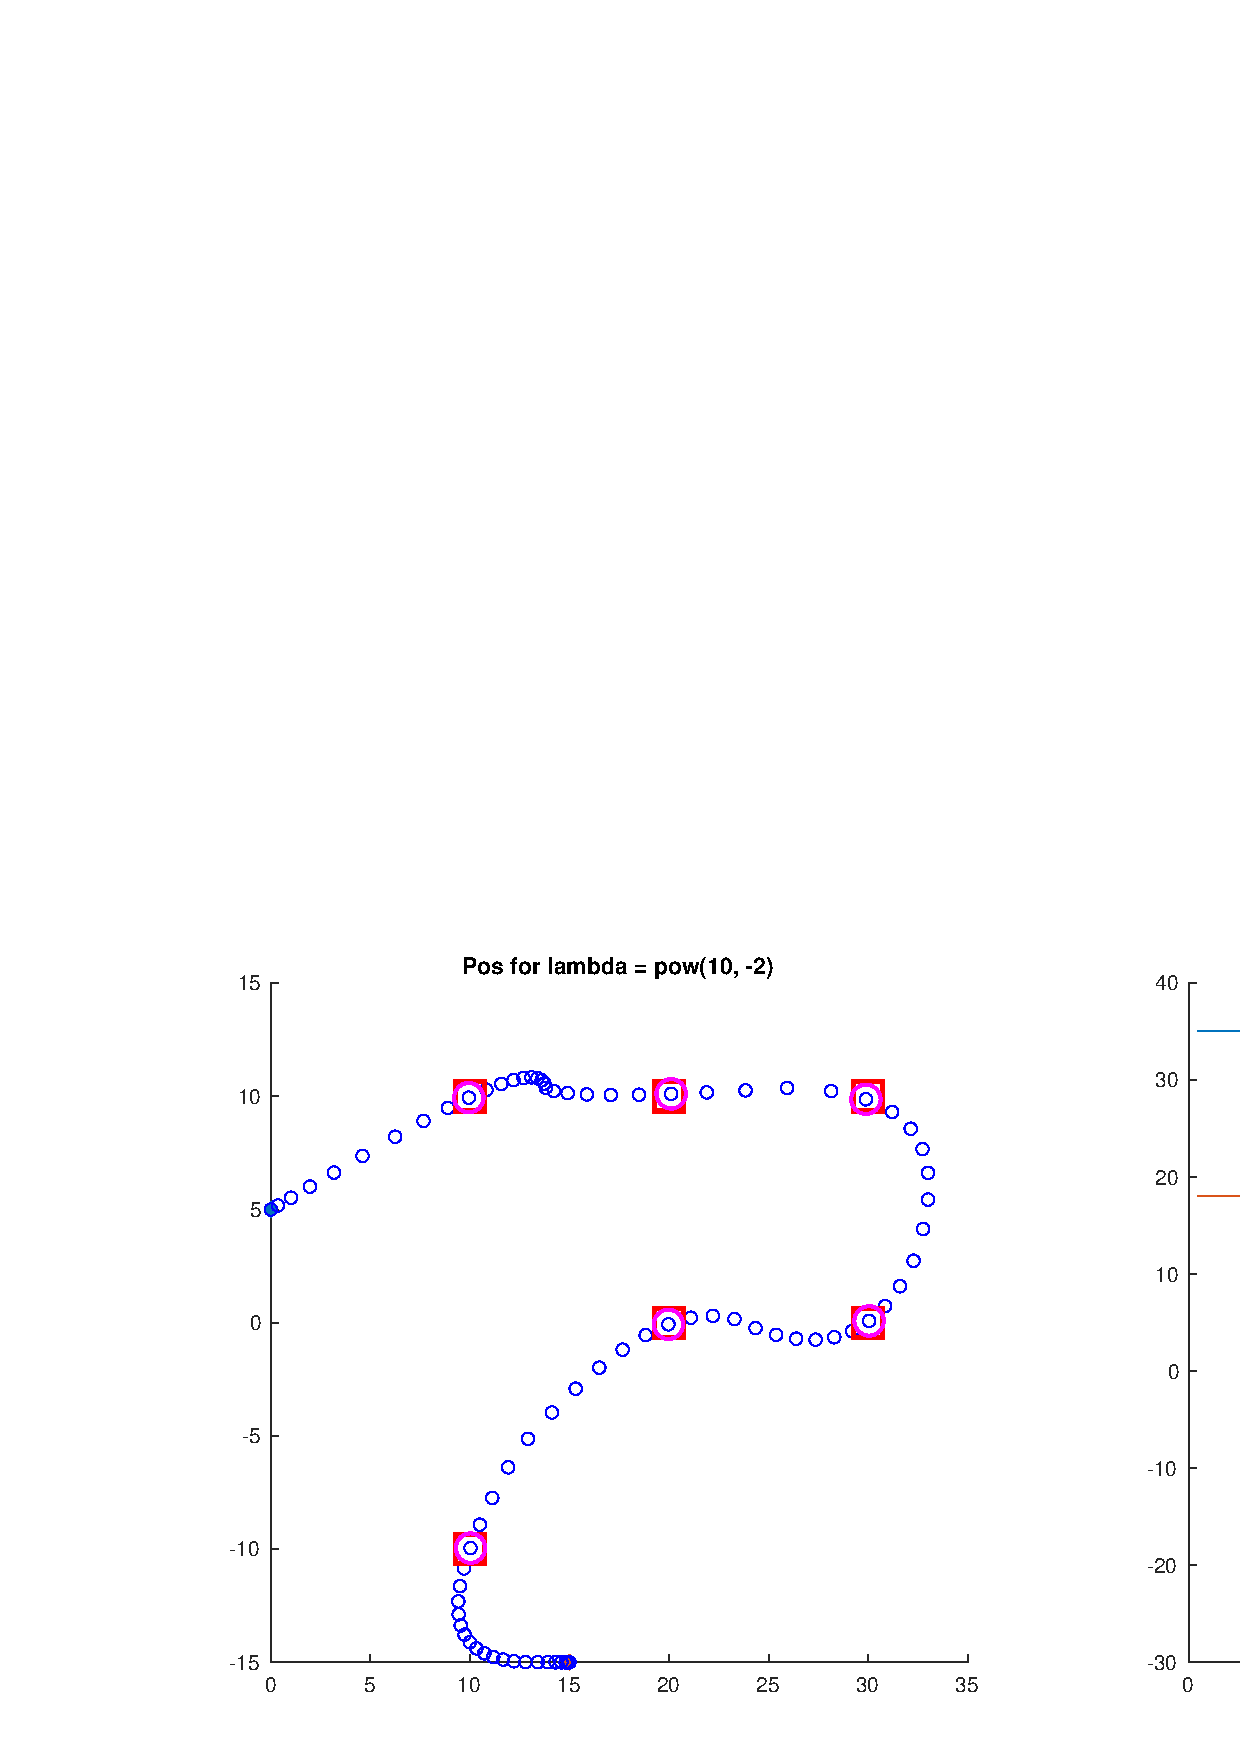
\includegraphics[width=0.5\linewidth]{part1/figures/task3/3_-2.pdf}
\end{subfigure}
\begin{subfigure}
    \centering
    \makebox[\linewidth]{%
        \hspace*{4px}
        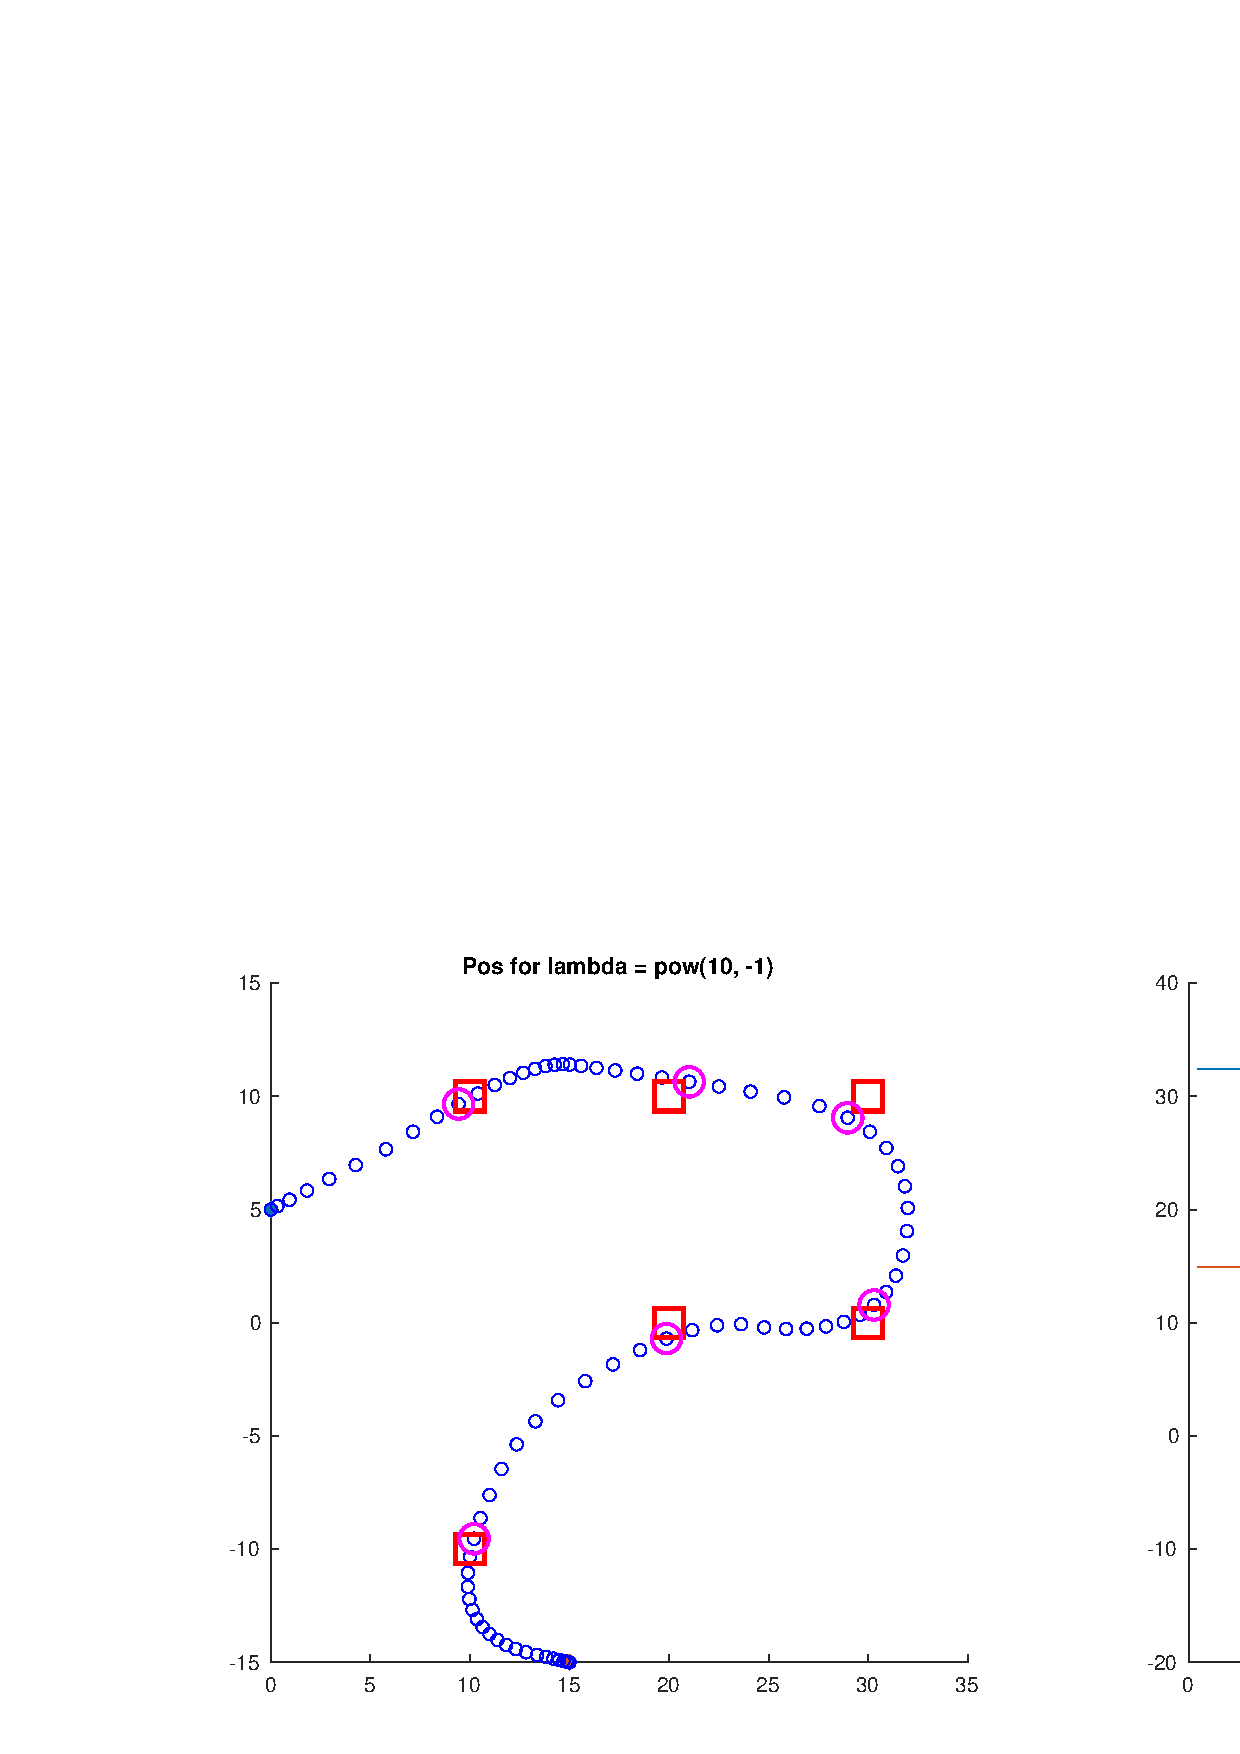
\includegraphics[width=\linewidth + 22px]{part1/figures/task3/3_-1.pdf}
    }
\end{subfigure}
\begin{subfigure}
    \centering
    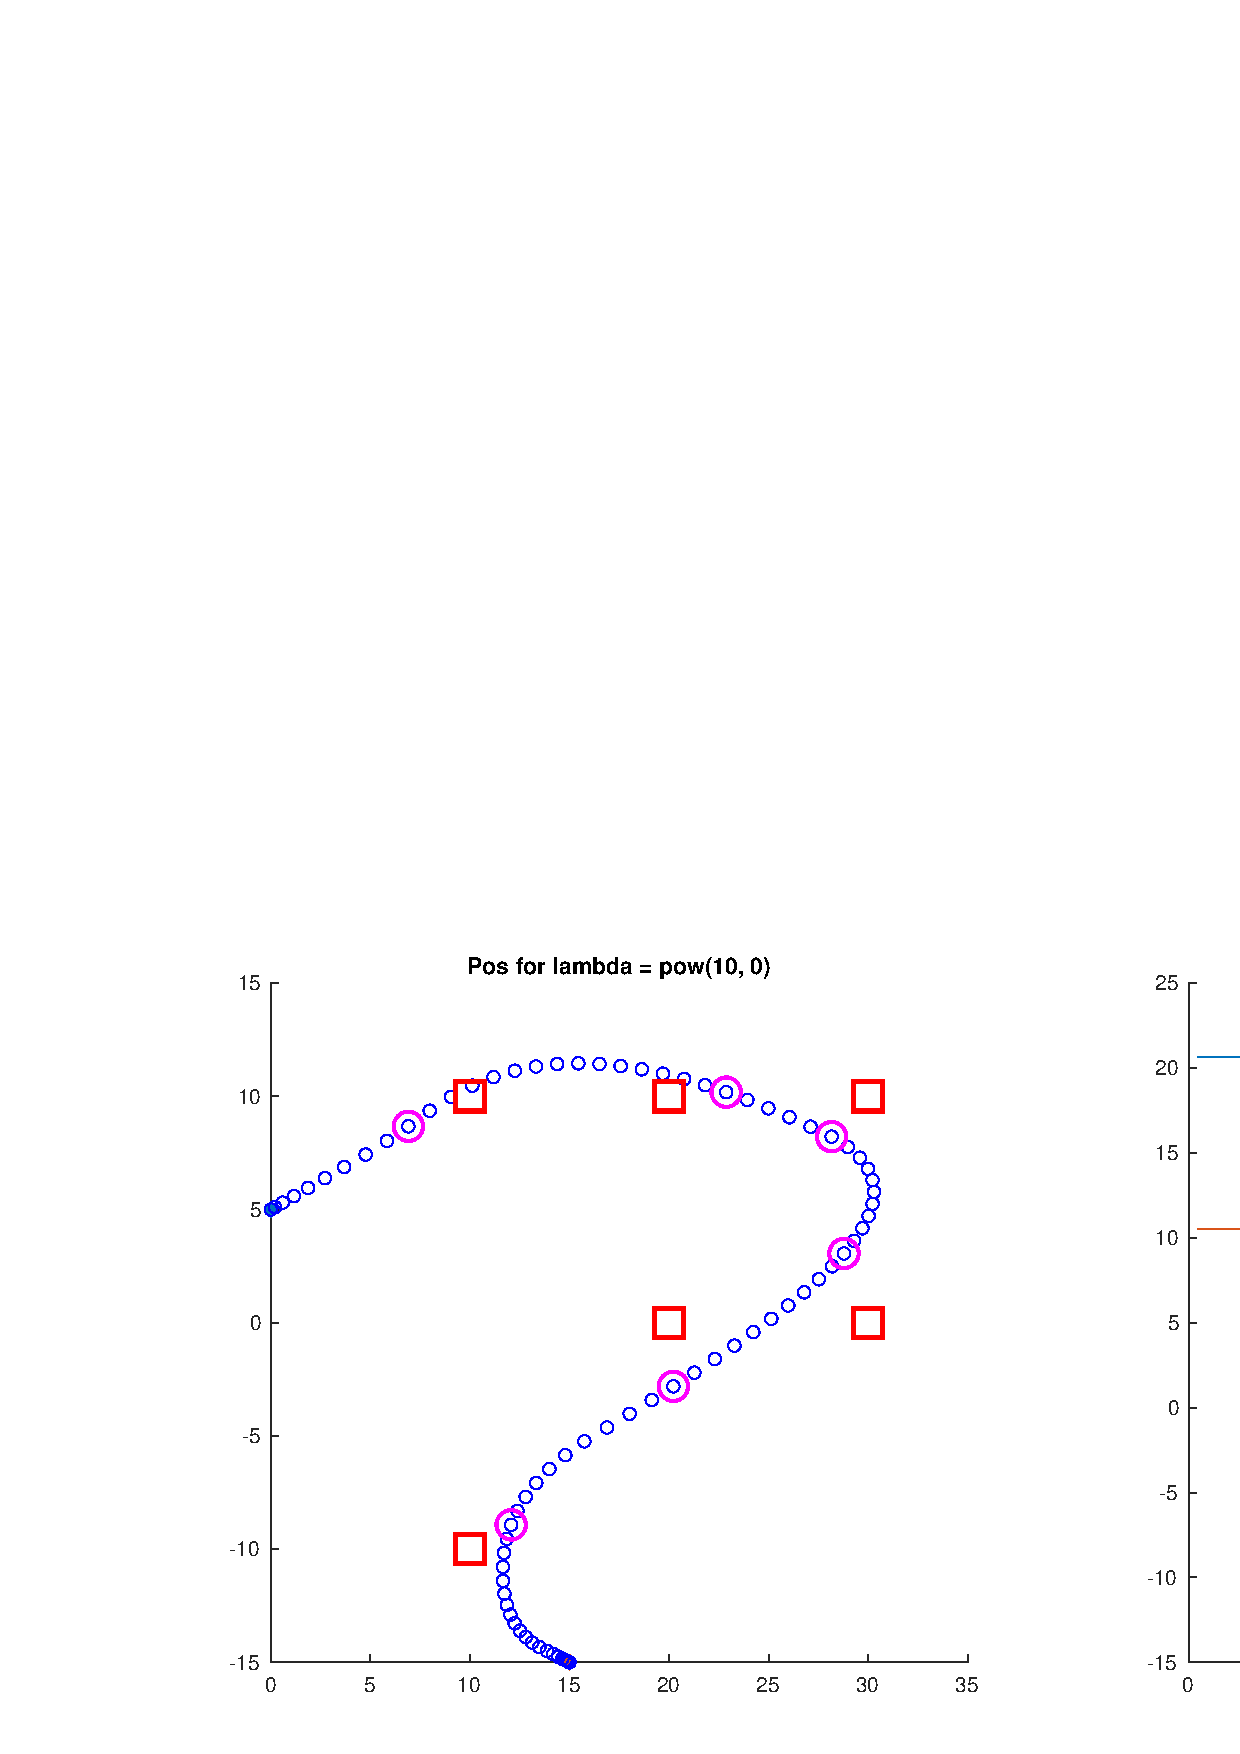
\includegraphics[width=0.5\linewidth]{part1/figures/task3/3_0.pdf}\hspace{0em}
    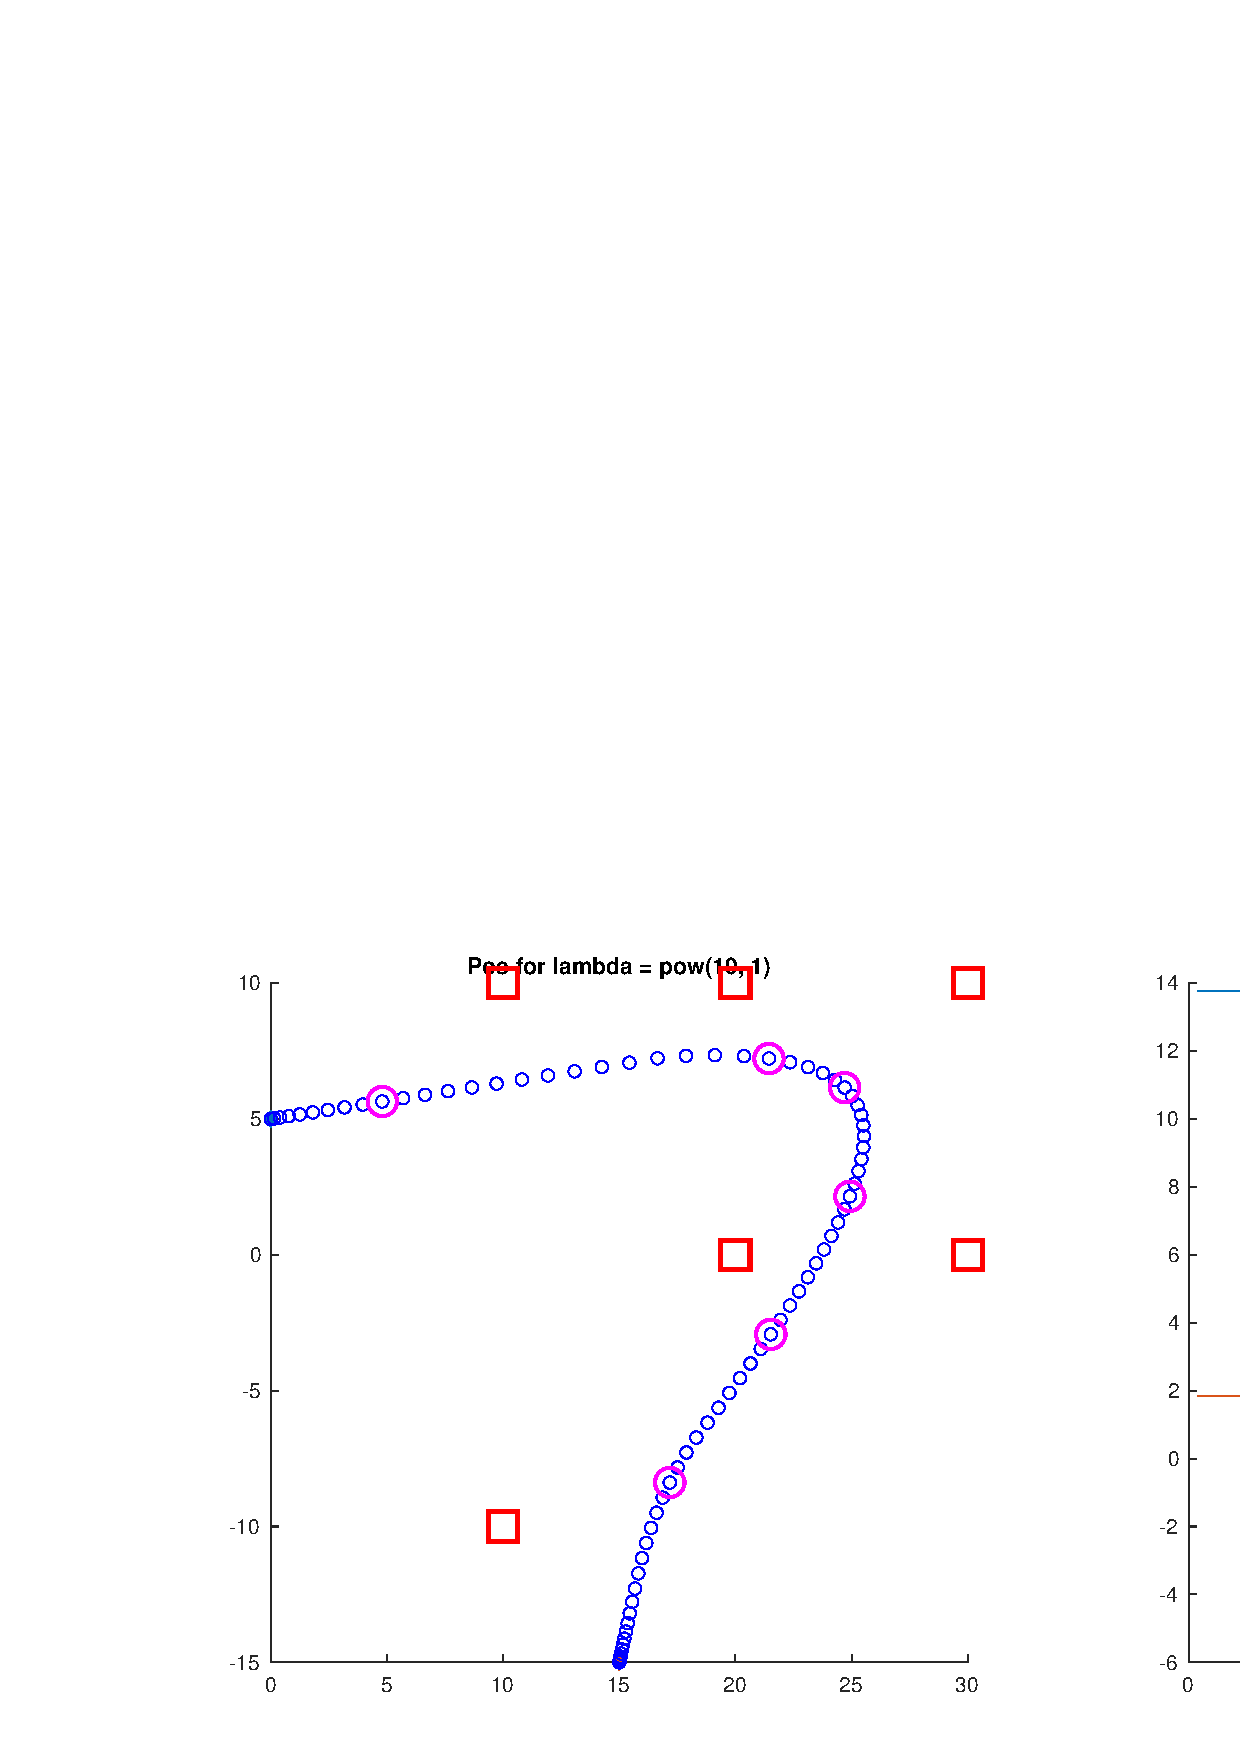
\includegraphics[width=0.5\linewidth]{part1/figures/task3/3_1.pdf}
\end{subfigure}
\begin{subfigure}
    \centering
    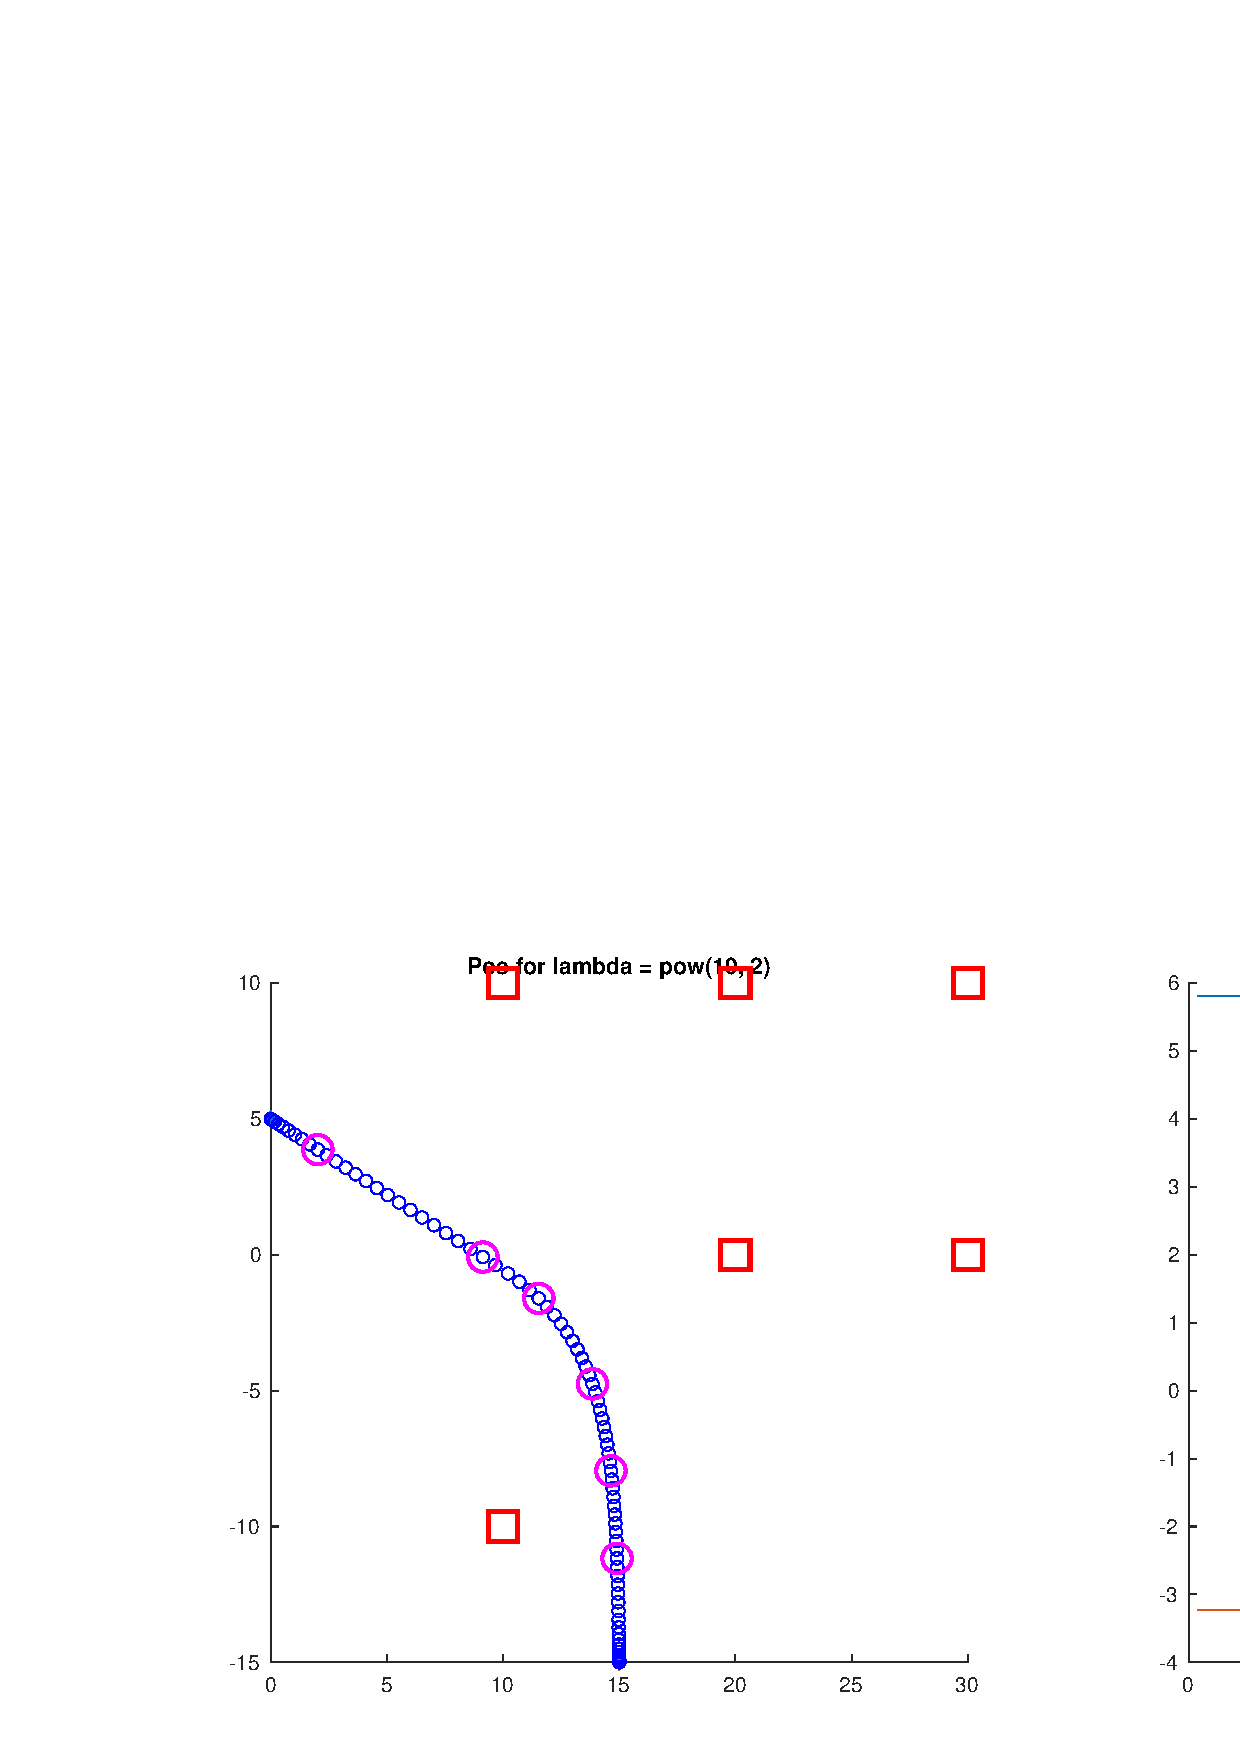
\includegraphics[width=0.5\linewidth]{part1/figures/task3/3_2.pdf}\hspace{0em}
    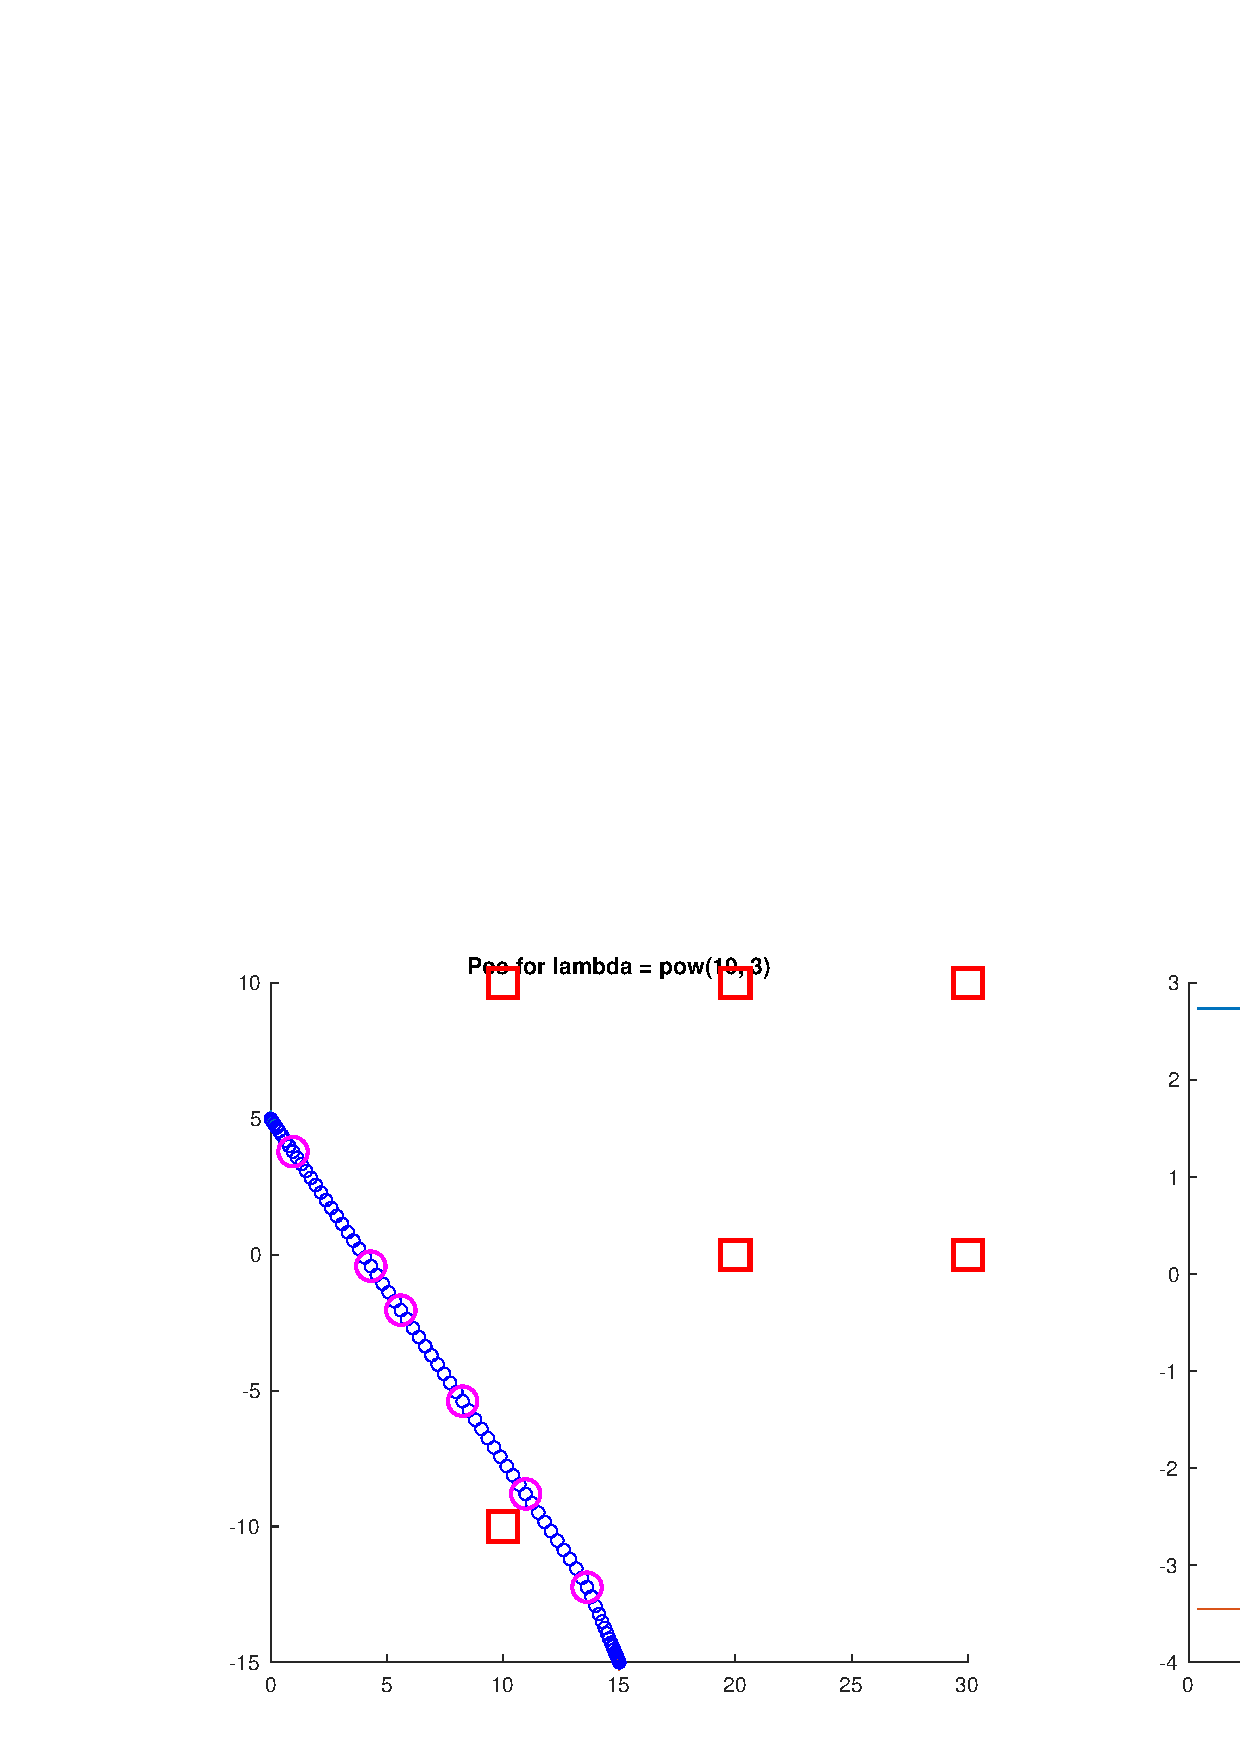
\includegraphics[width=0.5\linewidth]{part1/figures/task3/3_3.pdf}
\end{subfigure}
\caption{Robot positions and control signal for Task 3.}
\label{fig:task3:graphs}
\end{figure}

\clearpage
\subsection{Task 4}
%\noindent\fcolorbox{black}{lightgray}{
%    \parbox{\textwidth}{ \textbf{Task 4.} Comment on what you have observed from Tasks 1 to 3 (for example, compare the impact of the three regularizers on the optimal control signal that they each induce).
%    }
%}


\begin{table}[!htb]
    \caption*{Mean deviation and effect of the regularizer based on the $\lambda$ in Tasks 1 to 3.}
    \begin{minipage}{.33\linewidth}
        \centering
        \begin{tabular}{c|cr}
            $\lambda$ & changes & m. dev. \\
            \hline
            $10^{-3}$ & 79 & 0.1257 \\
            $10^{-2}$ & 79 & 0.8242 \\
            $10^{-1}$ & 79 & 2.1958 \\
            $10^{+0}$ & 79 & 3.6826 \\
            $10^{+1}$ & 79 & 5.6317 \\
            $10^{+2}$ & 79 & 10.9041 \\
            $10^{+3}$ & 79 & 15.3304
        \end{tabular}
        \caption{Task 1 results.}
        \label{task1:table:results}
    \end{minipage}%
    \begin{minipage}{.33\linewidth}
      \centering
        \begin{tabular}{c|cr}
            $\lambda$ & changes & m. dev. \\
            \hline
            $10^{-3}$ & 10 & 0.0075 \\
            $10^{-2}$ & 8 & 0.0747 \\
            $10^{-1}$ & 11 & 0.7021 \\
            $10^{+0}$ & 5 & 2.8876 \\
            $10^{+1}$ & 4 & 5.3689 \\
            $10^{+2}$ & 3 & 12.5914 \\
            $10^{+3}$ & 1 & 16.2266
        \end{tabular}
            \caption{Task 2 results.}
        \label{task2:table:results}
    \end{minipage}%
    \begin{minipage}{.33\linewidth}
      \centering
        \begin{tabular}{c|cr}
            $\lambda$ & changes & m. dev. \\
            \hline
            $10^{-3}$ & 13 & 0.0107 \\
            $10^{-2}$ & 12 & 0.1055 \\
            $10^{-1}$ & 14 & 0.8863 \\
            $10^{+0} $ & 11 & 2.8732 \\
            $10^{+1} $ & 6 & 5.4361 \\
            $10^{+2} $ & 2 & 13.0273 \\
            $10^{+3} $ & 2 & 16.0463
        \end{tabular}
        \caption{Task 3 results.}
        \label{task3:table:results}
    \end{minipage} 
\end{table}

The objective function which we try to minimize in the tasks 1 to 3 consists of sum of two parts. The first part, common to all of three tasks measures how far away the robot is from the waypoints at given times. This is defined as $\sum_{k = 1}^K \left\| E x( \tau_k ) - w_k \right\|_2^2$. 

Second part of the objective function, the regularizer, differs among the first three tasks. Regularizer enforces the fourth wish (simple control) by penalizing the deviations of the control signal from its previous value. By changing the $\lambda$ parameter, we can change the importance of this wish. If the $\lambda$ becomes a large number, the objective function's value shifts towards the regularizer which enforces least number of changes to the control signal. Making the $\lambda$ a large value naturally increases the mean deviation as we put larger importance to minimizing the number of changes of the control signal instead of capturing all of the points.

\noindent
\begin{minipage}{.33\linewidth}
    \begin{equation}
        \label{task1:regularizer}
        \sum_{t = 1}^{T-1} \left\| u(t) - u(t-1) \right\|_2^2
    \end{equation}
\end{minipage}
\begin{minipage}{.33\linewidth}
    \begin{equation}
        \label{task2:regularizer}
        \sum_{t = 1}^{T-1} \left\| u(t) - u(t-1) \right\|_2
    \end{equation}
\end{minipage}
\begin{minipage}{.33\linewidth}
    \begin{equation}
        \label{task3:regularizer}
        \sum_{t = 1}^{T-1} \left\| u(t) - u(t-1) \right\|_1
    \end{equation}
\end{minipage}

Effect of this behavior is shown in the Figure \ref{fig:task4:waypoint:dev}. The number of changes in the control signal does not change for the Task 1 as it stays $79$. The number of changes for Task 2 and 3 is visualized in the Figure \ref{fig:task4:changes}.


\begin{figure}[!htb]
    \centering
    \includegraphics[width=\linewidth]{part1/notebooks/task_2_3_signal_changes.pdf}
    \caption{Control signal changes for Tasks 2 and 3.}
    \label{fig:task4:changes}
\end{figure}


\begin{itemize}
    \item[\textbf{Task 1}] utilizes the squared L2 regularizer as shown in Equation \ref{task1:regularizer}. Benefit of using the squared L2 norm can be in easier computation, as no square root needs to be computed. The differences between control signals are absolutely limited by the \textit{U\_Max} constraint which results in them being often lower than 1. Squaring a small number leads to even smaller value. Since the value is too small, the contribution to the objective function is neglected and the optimizer rather optimizes capturing the waypoints. 
    \item[\textbf{Task 2}] utilizes the L2 norm, described in Equation \ref{task2:regularizer}. This can be interpreted as euclidean distance from the previous actuator vector to the current one. Calculating the square root of a small value ($<0$) makes this value larger. The contribution to the objective function is therefore larger than in the Task 1. The lowest number of updates (1) was achieved by using the $\lambda=10^3$. We can see, that the control signal's function is no longer smooth, but rather has a form of squares as the robot utilizes large control signals which change rarely.
    \item[\textbf{Task 3}] relies on the L1 norm, as described in Equation \ref{task3:regularizer}. This norm is not differentiable at 0, however it induces a behavior which was called ``L1 magic'' - the property of producing many coefficients with zero values or very small values with few large coefficients\footnote{http://www.chioka.in/differences-between-the-l1-norm-and-the-l2-norm-least-absolute-deviations-and-least-squares/}.
\end{itemize}

Surprisingly, the performance of the L2 norm in this task is superficial to the L1 norm as the robot achieves lower mean deviation with the same number of points captured. 

\begin{figure}[!htb]
    \centering
    \includegraphics[width=\linewidth]{part1/notebooks/task_1_2_3_waypoint_mean_dev.pdf}
    \caption{Waypoint mean deviation for Tasks 1 to 3.}
    \label{fig:task4:waypoint:dev}
\end{figure}

\subsection{Task 5}
%\noindent\fcolorbox{black}{lightgray}{
%    \parbox{\textwidth}{ \textbf{Task 5.} Using simple geometric arguments, give a  closed-form expression for $d\left( p,D(c,r) \right)$.
%    }
%}

Distance between point $p$ and disc $D\left(c, r\right)$ is defined as:
\begin{equation}
    d\left(p,D\left(c,r\right)\right) = \textit{min}\{\left\|p-y\right\|: y \in D\left(c, r\right)\}
\end{equation}

Based on whether the point is within the disc or not, the following cases might occur:
\begin{equation}
	d\left( p,D(c,r) \right) = 
	\begin{cases} 
		0                           & \text{if } \left\|p - c\right\|_2 \leq r\\ 
		\left\|p - c\right\|_2 - r 	& \text{if } \left\|p - c\right\|_2 > r
	\end{cases}
\end{equation}

If the result of $\left\|p - c\right\|_2 - r$ is negative, the point is within the circle and the distance should be 0. If the point is outside of the disc, then the result is equal to $\left\|p - c\right\|_2 - r$. Based on this, we conclude that the equation can be written in a closed form as:
\begin{equation}
    % \textit{max}\left(0, \left\|p(\tau_{k}), c_{k}\right\|_2 - r_k \right)
	d\left(p,D\left(c,r\right)\right) = \textit{max}\left(0, \left\|p - c\right\|_2 - r \right)
\end{equation}

\clearpage
\subsection{Task 6}
%\noindent\fcolorbox{black}{lightgray}{
%    \parbox{\textwidth}{ \textbf{Task 6.} Use the software ${\tt CVX}$ to solve problem~\eqref{P:prob4}. After you solve the problem, do the following:
%    \begin{enumerate}[(a)]
%    \item plot the optimal positions of the robot from $t = 0$ to $t = T$, marking its positions at the appointed times $\tau_k$, for $1 \leq k \leq K$;
%    \item plot the optimal control signal $u(t)$, where $u(t) = ( u_1(t), u_2(t) )$, from $t = 0$ to $t = T-1$;
%    \item report how many times the optimal control signal changes from $t = 1$ to $t = T-1$; 
%    \item report the mean deviation from the waypoints (defined in~\eqref{meanwaydev});     
%    \item comment on the results from (a)-(d), as you compare them with those you obtained in Task 1. (Note that Task 1 considered waypoints, which can be seen as disks with radius zero.)
%    \end{enumerate}
%    }
%}

% comment on the results from (a)-(d), as you compare them with those you obtained in Task 1. (Note that Task 1 considered waypoints, which can be seen as disks with radius zero.

Mean deviation and number of changes for the Task 6 is shown in the Table \ref{table:task6:table}. The resulting robot's optimal positions are shown in the Figure \ref{fig:task6:figure}. The snippet of the CVX code is shown in the Listing \ref{listing:task6:cvx}.

\begin{figure}[!htb]
    \centering    
    \includegraphics[width=1\linewidth]{part1/figures/task_6.pdf}
    \caption{Robot positions and control signal for Task 6.}
    \label{fig:task6:figure}
\end{figure}


The robot is now not rewarded for directly capturing the waypoint, it only needs to be within the disc's radius at the given time. With $\lambda=10^-1$ the robot achieves 8 changes as compared to 11 changes in the Task 2. The center mean deviation is $1.4141$ as compared to $0.7021$ achieved in the Task 2. We can see, that by not forcing the robot not to be at exact position at the given time, we have relaxed one of our wishes and as a tradeoff, the robot is able to achieve the task with lower number of signal changes. Of course, this comes at a cost of larger mean deviation.


\begin{table}[!htb]
    \label{table:task6:table}
    \begin{tabular}{c|ccr}
        $\lambda$ & changes & circle m. dev. & center m. dev. \\
        \hline
        $10^{-1}$ & 8 & 0 & 1.4142
    \end{tabular}
    \centering
    \caption{Mean deviation and number of changes for Task 6.}
\end{table}

\begin{lstlisting}[language=Matlab, caption=CVX code for task 6., label=listing:task6:cvx, float=!htb]
minimize(sum(max(0, vec_sqr_sum(c - x(1:2, tau+1)) - r))...
    + lambda*sum(norms(delta, 2)));
\end{lstlisting}


\subsection{Task 7}
%\noindent\fcolorbox{black}{lightgray}{
%    \parbox{\textwidth}{ \textbf{Task 7.} Use the software ${\tt CVX}$ to solve problem~\eqref{P:prob5a}. Explain what happens.}
%}

We implemented the task 7 in CVX code as shown in the listing \ref{listing:task7:cvx}. The variables are same as in the previous exercises with the exception of $\text{U\_Max}=15$.

\begin{lstlisting}[language=Matlab, caption=CVX code for task 7., label=listing:task7:cvx, float=!htb]
cvx_begin
    variable x(4,T+1);
    variable u(2,T);
    minimize(0);
    subject to
        % Initial and end speed need to be 0
        x(:,1)     == [p_initial; [0; 0]];
        x(:,T+1)   == [p_final;   [0; 0]];
        % Make sure that the robot moves using the constrains
        x(:,2:T+1) == A*x(:,1:T) + B*u(:,1:T);
        % Check the actuator force size
        for ux = u
            norm(ux, 2) <= U_max; 
        end
        % Enforce the correct positions of the robot
        for ti = 1:length(tau)
            E*x(:, tau(ti)) ==  w(:, ti);
        end
cvx_end
\end{lstlisting}

The CVX tries to solve this task, but fails to do so and reports the following:
\begin{lstlisting}
Status: Infeasible
Optimal value (cvx_optval): +Inf
\end{lstlisting}

This indicates, that CVX has not found a feasible solution to the given constrains. This is likely due to the actuator force $\text{U\_Max}=15$ being too low. 

We have investigated setting the \text{U\_Max} as another CVX variable and optimizing it with \lstinline{minimize(U_max)} which returns $38.8989$. We can see, that with value of $\text{U\_Max}=38.8989$ this feasibility problem has a solution.


\clearpage
\subsection{Task 8}
The function $\phi$ outputs zero if its argument is zero. Otherwise it outputs one. Function $\phi\,:\,{\mathbf R}^2 \rightarrow {\mathbf R}$, is defined as $$\phi(x) = \left\{ \begin{array}{ll} 0,  & \text{ if } x = 0, \\ 1, & \text{ if }x \neq 0. \end{array} \right.$$

%\noindent\fcolorbox{black}{lightgray}{
%    \parbox{\textwidth}{ \textbf{Task 8.} Show that the function $\phi$ is nonconvex.}
%}

\begin{equation}
	\forall x_1, x_2 \in X, \forall t \in [0, 1]: \qquad f(tx_1+(1-t)x_2)\leq t f(x_1)+(1-t)f(x_2)
\end{equation}

Function f is convex if for any two points $x_{1}, x_{2}$ and a parameter $t\in[0, 1]$ the above inequality is true. We select $x_{1} = 0$, $x_{2} = 1$ and $t=0.5$. The inequality for this setting and function $\phi$ is described below.

\begin{equation}
\begin{split}
	\phi(t \cdot x_1+(1-t) \cdot x_2) &\leq t \cdot \phi(x_1)+(1-t) \cdot \phi(x_2)\\
	\phi(0.5 \cdot 0 + 0.5 \cdot 1) &\leq 0.5 \cdot \phi(0) + 0.5 \cdot f(1)\\
	\phi(0.5) &\leq 0.5 \cdot \phi(0) + 0.5 \cdot f(1)\\
	1 &\leq 0.5
\end{split}
\end{equation}

As we can see above, this inequality is a contradiction for selected $x_{1}$, $x_{2}$ and t. Since $\phi$ does not fulfill the requirements for a convex function, we conclude that it is non convex.

\subsection {Task 9}
%\noindent\fcolorbox{black}{lightgray}{
%    \parbox{\textwidth}{ \textbf{Task 9.} Use the software ${\tt CVX}$ to solve problem~\eqref{P:prob6}. After you solve the problem, do the following:
%    \begin{enumerate}[(a)]
%    \item plot the optimal positions of the robot from $t = 0$ to $t = T$, marking its positions at the appointed times $\tau_k$, for $1 \leq k \leq K$;
%    \item plot the optimal control signal $u(t)$, where $u(t) = ( u_1(t), u_2(t) )$, from $t = 0$ to $t = T-1$;
%    \item report how many waypoints are captured by the robot; consider that a waypoint $w_k$ is captured if the robot is sufficiently close to it at the appointed time $\tau_k$, namely, if $\left\| p( \tau_k) - w_k \right\|_2 \leq 10^{-6}$.
%    \end{enumerate}
%    }
%}

The minimized function can be expressed in CVX as shown on Listing \ref{listing:task9:cvx}.

\begin{lstlisting}[language=Matlab, caption=CVX code for task 9., label=listing:task9:cvx]
minimize(sum(vec_sqr_sum(E*x(:,tau+1) - w)));
\end{lstlisting}

The robot positions are shown in the Figure \ref{fig:task9:graph}. The robot did not capture any point.

\begin{figure}[!htb]
    \centering    
    \includegraphics[width=1\linewidth]{part1/figures/task_9.pdf}
    \caption{Robot positions and control signal for Task 9.}
    \label{fig:task9:graph}
\end{figure}

\subsection {Task 10}
%\noindent\fcolorbox{black}{lightgray}{
%    \parbox{\textwidth}{ \textbf{Task 10.} Redo task 9 for problem~\eqref{P:prob7}.
%    }
%}

The minimized function can be expressed in CVX as shown on Listing \ref{listing:task10:cvx}. The robot has captured a single point along its journey.

\begin{lstlisting}[language=Matlab, caption=CVX code for task 10., label=listing:task10:cvx]
minimize(sum(norms(E*x(:,tau+1) - w, 2)));
\end{lstlisting}

The resulting robot positions are visualized in the Figure \ref{fig:task10:graph}.

\begin{figure}[!htb]
    \centering    
    \includegraphics[width=1\linewidth]{part1/figures/task_10.pdf}
    \caption{Robot positions and control signal for Task 10.}
    \label{fig:task10:graph}
\end{figure}

\clearpage
\subsection {Task 11}
%\noindent\fcolorbox{black}{lightgray}{
%    \parbox{\textwidth}{ \textbf{Task 11.} Apply the reweighting  technique $M$ times, with $M = 10$; that is, solve problem problem~\eqref{P:prob8} for $m = 0, 1, \ldots, M-1$. For each value of $m$, do the following:
%     \begin{enumerate}[(a)]
%    \item plot the positions of the robot in $x^{(m)}$ from $t = 0$ to $t = T$, marking its positions at the appointed times $\tau_k$, for $1 \leq k \leq K$;
%    \item plot the control signal $u^{(m)}(t)$, where $u^{(m)}(t) = \left( u_1^{(m)}(t), u_2^{(m)}(t) \right)$, from $t = 0$ to $t = T-1$;
%    \item report how many waypoints are captured by the robot.
%    \end{enumerate}}
%}

The solution to the reweighting problem is visualized in the Figure \ref{fig:task11:graphs}. The results are described in the Table \ref{table:task11:results}.

\begin{table}[!htb]
\centering
\begin{tabular}{l|ll}
m & captured & mean deviation \\
\hline
0 & 1 & 2.4157 \\
1 & 2 & 2.4567 \\
2 & 2 & 2.5737 \\
3 & 3 & 2.7362 \\
4 & 3 & 2.7355 \\
5 & 3 & 2.7355 \\
6 & 3 & 2.7355 \\
7 & 3 & 2.7355 \\
8 & 3 & 2.7355 \\
9 & 3 & 2.7355
\end{tabular}
\caption{Results of the reweighting technique in Task 11.}
\label{table:task11:results}
\end{table}

\begin{figure}[!htb]
    \begin{subfigure}
        \centering
        \includegraphics[width=0.5\linewidth]{part1/figures/task11/task_11_0.pdf}\hspace{0em}
        \includegraphics[width=0.5\linewidth]{part1/figures/task11/task_11_1.pdf}
    \end{subfigure}
    \begin{subfigure}
        \centering
        \includegraphics[width=0.5\linewidth]{part1/figures/task11/task_11_2.pdf}\hspace{0em}
        \includegraphics[width=0.5\linewidth]{part1/figures/task11/task_11_3.pdf}
    \end{subfigure}
    \begin{subfigure}
        \centering
        \includegraphics[width=0.5\linewidth]{part1/figures/task11/task_11_4.pdf}\hspace{0em}
        \includegraphics[width=0.5\linewidth]{part1/figures/task11/task_11_5.pdf}
    \end{subfigure}
    \begin{subfigure}
        \centering
        \includegraphics[width=0.5\linewidth]{part1/figures/task11/task_11_6.pdf}\hspace{0em}
        \includegraphics[width=0.5\linewidth]{part1/figures/task11/task_11_7.pdf}
    \end{subfigure}
    \begin{subfigure}
        \centering
        \includegraphics[width=0.5\linewidth]{part1/figures/task11/task_11_8.pdf}\hspace{0em}
        \includegraphics[width=0.5\linewidth]{part1/figures/task11/task_11_9.pdf}
    \end{subfigure}
    \caption{Robot positions and control signal for Task 11.}
    \label{fig:task11:graphs}
\end{figure}

\subsection {Task 12}
%\noindent\fcolorbox{black}{lightgray}{
%    \parbox{\textwidth}{ \textbf{Task 12.} What's the role of the weights in~\eqref{P:prob8}?
%}}

The optimizer tries to optimize the utility function of each waypoint divided by the previous value. The utility values for first 5 iterations are shown in Listing \ref{task12:listing:results}.

\begin{lstlisting}[label=task12:listing:results, caption=Unweighted utility function for each waypoint., float=!htb]
    5.9580    0.9926    3.3379    1.8267    2.3790    0.0000
    6.0346    0.0000    4.3660    1.3281    3.0118         0
    6.0892         0    4.4750    0.3854    4.4923         0
    6.2897         0    4.4125    0.0000    5.7152         0
    6.2540         0    4.3987    0.0000    5.7602         0
    6.2514         0    4.3983    0.0000    5.7630         0
    6.2512         0    4.3983    0.0000    5.7632         0
    6.2512         0    4.3983    0.0000    5.7632         0
    6.2512         0    4.3983    0.0000    5.7632         0
    6.2512         0    4.3983    0.0000    5.7632         0
\end{lstlisting}

By investigating the resulting utility function sizes for each waypoint, we can see that if the robot captures the waypoint, the utility becomes $0$. Since the optimizer tries to minimize the sum of the utility function for each waypoint, thanks to the reweighting technique, it already has the information that the waypoint can be captured (in form of the previous iteration's utility value). The previous utility value was $0$ and when we divide any number by a very small number ($\epsilon = 10^{-6}$) this fraction explodes thus forcing the optimizer to keep this value small by setting the numerator $0$ again. 

\section{Part 2}
In this part, it is required to minimize $f(s,r)$, represented in equation \ref{log_regression},using various methods to give optimal values of (s,r).
\begin{equation}
    \label{log_regression}
    f(s,r)=\sum_{k=1}^{K}\log(1+ \exp(s^{T}x_k - r)) - y_k(s^{T}x_k - r)
\end{equation}
\subsection{Task 1}
To prove the convexity of the function, it is easier to breakdown function F, in equation \ref{log_regression} and figure \ref{pt2task1:conv} as a composition of smaller functions: \begin{equation}
   \begin{split}
    F &= F_1 + \hdots + F_k  \\ 
F_1 &= G_1 + H_1 \\
G_1 &= Q_1(F_1)
\end{split}
\end{equation}
Where \begin{equation}
   \begin{split}
   H_1&= -y_1(s^{T}x_1-r)\\
   P_1&= s^{T}x_1 - r  \\
   Q_1 &= log(1+ e^z)\\
   \end{split}
\end{equation}
$P_1$ can be expressed as an inner product between the vector of variables (s,r) (equation \ref{P_1}) and the vector constants $x_1$ . This is also the trick used in the implementation of the Gradient and Newton methods, so that only matrix and vector calculations take place. It is affine, therefore convex.
\begin{equation}
\label{P_1}
\begin{bmatrix} x_1^{T} & -1\end{bmatrix} \begin{bmatrix} s \\
                                                           r
                                                           \end{bmatrix}
\end{equation}
The composed function $Q_1(F_1)$ is convex, because $\ddot Q_1(z) > 0, \forall z \in \mathbb{R}$.\\ 
The same thought process of equation \ref{P_1} can be applied to $H_1$, but in this case the constants also take into account $y_1$. The sum of a convex function to another  ($H_1 + G_1$) only changes the offset of the function images, so it still remains convex.
\begin{equation}
\label{H_1}
\begin{bmatrix} -y_1x_1^{T} & y_1\end{bmatrix} \begin{bmatrix} s \\
                                                           r
                                                           \end{bmatrix}
\end{equation}
If $F_1$ is convex, then all of the $F_k$ are convex too, since all of them have the same structure. Therefore, their sum is also convex, making F a convex function.
\begin{figure}[H]
	\centering
	\includegraphics[width=0.5\linewidth]{part2/figures/Convex.png}
	\caption{Schematic breakdown of $f(s,r)$, represented by F} \label{pt2task1:conv}		
\end{figure}
\subsection{Task 2}
The code for the Gradient method can be observed at listing \ref{listing:pt2task2:gradient}. It is worth noticing that a strategy like equation \ref{P_1} was enforced, so as to simplify and optimize the calculations, without for-loops.
\begin{lstlisting}[language=Matlab, caption=Matlab code for the Gradient method., label=listing:pt2task2:gradient]
function [S] = grad_descent_2(X,Y,s0,r0,e)
%grad_descent_2 applies the gradient method
%   Inputs : X,Y,e= dataset,labels,error tolerance
%            s0,r0= initial s, initial r
%   Outputs: S = [X_features+1]*[k] matrix, where S(:,end) is the final
%            value; [S(1:end-1,:); S(end,:)]= [values of s ; values of r] 
%            troughout the method
k=1;
%Compactly defines an affine mapping, so that matricial notation can be
%employed . [s;r]'*[x;-1] = s'*x - r 
S(:,1)=[s0;r0];
X(end+1,:)=-1;
%define functions f, and its first derivative in order of s'*x
d_f=@(x,s,y)(exp(s'*x)./(1+exp(s'*x))) - y ;
f=@(x,s,y) sum(log(1+ exp(s'*x)) - y.*(s'*x))/length(x);
while(1)
    %calculate gradient
    g=(X*(d_f(X,S(:,k),Y)'))/length(X);
    grad_norm(k)=norm(g);
    if(norm(g) < e)
        break;
    else
        d=-g;
        %backtracking routine
        a(k)=1;
        while(1)
            cond2= f(X,S(:,k),Y)+(10^-4)*g'*(a(k)*d);
            cond1= f(X,S(:,k)+a(k)*d,Y);
            if(cond1<cond2)
                break;
            end
            %step size recalculation
            a(k)=a(k)*0.5;
        end
        % calculation of k(th) iteration of the values of s and r 
        S(:,k+1)=S(:,k)+a(k)*d;
        k=k+1;
    end
end
%Norm graph
figure
semilogy(1:k,grad_norm);
xlabel('$k$','interpreter','latex')
title('$||\nabla{f(s_k,r_k)}||$ (Gradient Method)','interpreter','latex')
grid on;
end

\end{lstlisting}
\begin{figure}[!htb]
	\centering
	\includegraphics[width=0.5\linewidth]{part2/figures/T2_Line.png}
	\caption{\texttt{data1.mat} (blue,red) with optimized hyperplane (green) using Gradient method}\label{pt2task2:graph}		
\end{figure}
\begin{figure}[!htb]
		\centering
		\includegraphics[width=0.5\linewidth]{part2/figures/T2_Norm.png}
		\caption{\texttt{data1.mat} $||\nabla{f(s_k,r_k)}||$ evolution}\label{pt2task2:Norm}	
\end{figure}
    
\subsection{Task 3}

\begin{figure}[H]
	\centering
	\includegraphics[width=0.5\linewidth]{part2/figures/T3_Line.png}
	\caption{\texttt{data2.mat} (blue,red) with optimized hyperplane (green) using Gradient method}\label{task3:graph}		
\end{figure}

\begin{figure}[!htb]
		\centering
		\includegraphics[width=0.5\linewidth]{part2/figures/T3_Norm.png}
		\caption{\texttt{data2.mat} $||\nabla{f(s_k,r_k)}||$ evolution}\label{fig:pt2task3:Norm}	
\end{figure}

\begin{table}[H]
\centering
\begin{tabular}{l|lll}
 & $s_1$ & $s_2$ & $r$ \\ \hline
data1.mat & 1.3495 & 1.0540 & 4.8815 \\
data2.mat & 0.7402 & 2.3577 & 4.5553
\end{tabular}
\caption{Gradient method values of $s$ and $r$ for tasks 2 and 3.}
\label{table:task3:results}
\end{table}
\subsection{Task 4}
\begin{figure}[H]
    \label{fig:pt2task4:graphs}
    \begin{subfigure}
        \centering
        \includegraphics[width=0.45\linewidth]{part2/figures/T4_Norm_data3.png}\hspace{0em}
        \includegraphics[width=0.45\linewidth]{part2/figures/T4_Norm_data4.png}
    \end{subfigure}
    \caption{\texttt{data3.mat} (left) and \texttt{data4.mat} (right) $||\nabla{f(s_k,r_k)}||$ evolution}
\end{figure}


\subsection{Task 5}
Given $p(x) = \sum_{k=1}^{K} \phi(a_k^{T}x)$ where $ \phi : R\to R$ is a twice differentiable function.\\
To compute the gradient of the function, $\nabla{p(x)}$, chain rule of differentiation can be used :
\begin{equation}
 \nabla{p(x)}= \sum_{k=1}^{K} \frac{\partial \phi(a_k^{T}x)}{\partial a_k^{T}x} \cdot \frac{\partial a_k^{T}x}{\partial x}
\end{equation} 
\begin{equation}
\sum_{k=1}^{K} \frac{\partial \phi(a_k^{T}x)}{\partial a_k^{T}x} \cdot \frac{\partial a_k^{T}x}{\partial x} = \sum_{k=1}^{K}  \dot\phi(a_k^{T}x)\cdot a_k^{T} = \sum_{k=1}^{K} a_k\dot\phi(a_k^{T}x) = [a_1  a_2 \hdots a_k] \begin{bmatrix} \dot\phi(a_1^{T}x) \\
                                                           \dot\phi(a_2^{T}x) \\
                                                           \vdots \\
                                                           \dot\phi(a_k^{T}x)
                                                           \end{bmatrix}
\end{equation} 
We can then simplify to:
\begin{equation}
Av = [a_1  a_2 \hdots a_k] \begin{bmatrix} \dot\phi(a_1^{T}x) \\
                                                           \dot\phi(a_2^{T}x) \\
                                                           \vdots \\
                                                           \dot\phi(a_k^{T}x)
                                                           \end{bmatrix}= \nabla{p(x)}
\end{equation}
With dimensions $3\times1$, since A is $3\times K$ and $v$ is $K\times1$\\
To prove the structure of $\nabla^{2}{p(x)}$ we are going to refer once more to the chain rule of derivation, keeping in mind some concepts used in former passages:
\begin{equation}
\nabla^{2}{p(x)}= \frac{\partial Av}{\partial v} \cdot \frac{\partial v}{\partial x} = A \cdot AD%\begin{bmatrix} \ddot\phi(a_1^{T}x) \\
                          %                                \ddot\phi(a_2^{T}x) \\
                           %                                \vdots \\
                           %                                \ddot\phi(a_K^{T}x)
                           %                                \end{bmatrix} 
\end{equation}
The Hessian matrix has to have $3\times3$ dimensions. 
It just so happens that the term on the right of the dot product in the result has the same dimensions as the gradient, which will invert, since we have a dot product. 
Knowing that $\ddot\phi(a_k^{T}x)$ is a scalar the second term looks very much like a multiplication between a vector and a diagonal matrix.\\Thus we can elaborate more of the structure 
\begin{equation}
A \cdot AD = AD^{T}A^{T} = ADA^{T}
\end{equation}
With D being, in this specific case:
\begin{equation}
\begin{bmatrix}
 \ddot\phi(a_1^{T}x)&  & &\\
 &\ddot\phi(a_2^{T}x) & &\\ 
 &  &\ddots &\\ 
 &  & &\ddot\phi(a_k^{T}x)
\end{bmatrix}
\end{equation}
\subsection{Task 6}
The code for the Gradient method can be observed at listing \ref{listing:pt2task6:Newton}.
\begin{lstlisting}[language=Matlab, caption=Matlab code for the Newton method., label=listing:pt2task6:Newton]
function [ S ] = Newton_method( X,Y,s0,r0,e )
%Newton_method applies the newton method
%   Inputs : X,Y,e= dataset,labels,error tolerance
%            s0,r0= initial s, initial r
%   Outputs: S = [X_features+1]*[k] matrix, where S(:,end) is the final
%            value; [S(1:end-1,:); S(end,:)]= [values of s ; values of r] 
%            troughout the method
k=1;
%Compactly defines an affine mapping, so that matricial notation can be
%employed . [s;r]'*[x;-1] = s'*x - r  
S(:,1)=[s0;r0];
X(end+1,:)=-1;
%define functions f, and its first and second derivatives in order of s'*x
f=@(x,s,y) (1/length(x))*sum(log(1+ exp(s'*x)) - y.*(s'*x));
d_f=@(x,s,y)(exp(s'*x)./(1+exp(s'*x))) - y ;
h=@(x,s) exp(s'*x)./((1+exp(s'*x)).^2) ;

while(1)
    %calculate gradient
    g= X*(d_f(X,S(:,k),Y))'/length(X);
    grad_norm(k)=norm(g);
    if(norm(g) < e) 
        break;
    else
        %calculate hessian
        hess= X*diag(h(X,S(:,k)))*X'/length(X);
        d= -(hess)^-1*g;
        %backtracking routine
        a(k)=1;
        while(1)
            cond2= f(X,S(:,k),Y)+(10^-4)*g'*(a(k)*d);
            cond1= f(X,S(:,k)+a(k)*d,Y);
            if(cond1<cond2)
                break;
            end
            %step size recalculation
            a(k)=a(k)*0.5;
        end
        % calculation of k(th) iteration of the values of s and r 
        S(:,k+1)=S(:,k)+a(k)*d;
        k=k+1;
    end
end

%Norm graph
figure
semilogy(1:k,grad_norm);
xlabel('$k$','interpreter','latex')
xlim([1 k]);
title('$||\nabla{f(s_k,r_k)}||$ (Newton method)','interpreter','latex')
grid on;
%stepsize graph
figure
stem(a,'filled');
xlabel('$k$','interpreter','latex')
title('$ \alpha_k$ (Newton method)','interpreter','latex')
xlim([1 k-1]);
ylim([0 max(a)]);
end

\end{lstlisting}

\begin{figure}[H]
\label{fig:pt2task6:data1line}
        \centering
        \includegraphics[width=0.5\linewidth]{part2/figures/T6_Line_data1.png}
        \caption{\texttt{data1.mat} (blue,red) with optimized hyperplane (green) using Newton method}
\end{figure}

\begin{figure}[H]
    \label{fig:pt2task6:data1}
    \begin{subfigure}
        \centering
        \includegraphics[width=0.45\linewidth]{part2/figures/T6_Norm_data1.png}\hspace{0em}
        \includegraphics[width=0.45\linewidth]{part2/figures/T6_stepsize_data1.png}
       
    \end{subfigure}
    \caption{\texttt{data1.mat} $||\nabla{f(s_k,r_k)}||$ (left) and step size (right) evolution}
\end{figure}

\begin{figure}[H]
\label{fig:pt2task6:data2line}
        \centering
        \includegraphics[width=0.5\linewidth]{part2/figures/T6_Line_data2.png}
          \caption{data2.mat (blue,red) with optimized hyperplane (green) using Newton method}
\end{figure}

\begin{figure}[H]
    \label{fig:pt2task6:data2}
    \begin{subfigure}
        \centering
        \includegraphics[width=0.45\linewidth]{part2/figures/T6_Norm_data2.png}\hspace{0em}
        \includegraphics[width=0.45\linewidth]{part2/figures/T6_stepsize_data2.png}
       
    \end{subfigure}
    \caption{data2.mat $||\nabla{f(s_k,r_k)}||$ (left) and step size (right) evolution}
\end{figure}
\begin{table}[]
\centering
\begin{tabular}{l|lll}
 & s\_1 & s\_2 & r \\ \hline
data1.mat & 1.3496 & 1.0540 & 4.8817 \\
data2.mat & 0.7402 & 2.3577 & 4.5554
\end{tabular}
\caption{Newton method values of $s$ and $r$ for data1.mat and data2.mat.}
\label{table:task6:results}
\end{table}
\begin{figure}[H]
    \label{fig:pt2task6:data3}
    \begin{subfigure}
        \centering
        \includegraphics[width=0.45\linewidth]{part2/figures/T6_Norm_data3.png}\hspace{0em}
        \includegraphics[width=0.45\linewidth]{part2/figures/T6_stepsize_data3.png}
       
    \end{subfigure}
    \caption{data3.mat gradient norm (left) and step size (right) evolution}
\end{figure}

\begin{figure}[H]
    \label{fig:pt2task6:data4}
    \begin{subfigure}
        \centering
        \includegraphics[width=0.45\linewidth]{part2/figures/T6_Norm_data4.png}\hspace{0em}
        \includegraphics[width=0.45\linewidth]{part2/figures/T6_stepsize_data4.png}
       
    \end{subfigure}
    \caption{data4.mat $||\nabla{f(s_k,r_k)}||$ (left) and step size (right) evolution}
\end{figure}
\subsection{Task 7}
As can be consistently seen throughout the results, the Newton method converges in quite less iterations than the gradient method. This happens because in each iteration of the Newton method, the direction of the step and stepsize are calculated with a second order approximation of the function to minimize, which in its turn allows for a faster convergence on the long run.It was also a faster method time-wise, mainly due to the data sets tested. \\ We do believe that the time-wise results would favor the gradient method in datasets with very large number of features of X, mainly due to the complexity of the Gradient and Newton methods ($\mathcal{O}(n)$ and $\mathcal{O}(n^{3})$, respectively).\\
The Gradient method also has an advantage in terms of computational cost (space used) in each iteration, so it has a lot better performance when its used in situations like deep learning, where milions of parameters exist. That is why it is a better alternative to the Newton method, in these specific cases. If you have low to reasonable number of features and enough memory space, it's favourable to go for the Newton method.
\subsection{Task 8}

The code for the 8th task is in Listing \ref{listing:task8:lm} and the results obtained after running it for the \texttt{lmdata1.m} dataset are in Figs. \ref{fig:task8:netloc} and \ref{fig:task8:norm}.

\begin{lstlisting}[language=Matlab, caption=Matlab code for task 8., label=listing:task8:lm]
function [result, f_est] = lm(dataset, xinit, print)
    load(dataset, 'A', 'iA', 'y', 'z', 'iS', 'S');
    
    clc; 
    close all
    xk = xinit;

    % because vecnorm(x, dim) isn't available before R2017a
    vnorm = @(mat, dim) sqrt(sum(mat.^2, dim));

    % represents sp - sq
    sel = [1 0 -1 0; 0 1 0 -1];

    norms_f = [];
    lambda = 1;
    epsilon = 10^(-6);
    while 1
        [am, sp1, sp2, sq] = variables(xk, iA, A, iS);

        [f, fa, fs] = fx(am, sp1, sp2, sq, y, z);

        grad_fa = zeros(size(am, 1), length(xk));
        for ii = 1:length(iA)
            grad_fa(ii, [2*iA(ii,2)-1 2*iA(ii,2)]) = ...
            (sp1(ii,:) - am(ii,:)) ./ vnorm(am(ii,:) - sp1(ii,:), 2);
        end

        grad_fs = zeros(size(sq, 1), length(xk));
        for ii = 1:length(iS)
            grad_fs(ii, [2*iS(ii,1)-1 2*iS(ii,1) ...
                2*iS(ii,2)-1 2*iS(ii,2)]) = ((sel'*sel*[sp2(ii,:) ...
                sq(ii,:)]') ./ vnorm(sp2(ii,:) - sq(ii,:), 2))';
        end

        g_k = [2.*grad_fa.*fa; 2.*grad_fs.*fs];
        norm_gk = norm(sum(g_k, 1));

        norms_f = [norms_f norm_gk];
        if norm_gk < epsilon
           break; 
        end 

        x_est = [grad_fa; grad_fs; sqrt(lambda).*eye(size(g_k,2))]...
            \ [grad_fa*xk - fa; grad_fs*xk - fs; sqrt(lambda) * xk];

        [am, sp1, sp2, sq] = variables(x_est, iA, A, iS);
        [f_est, ~, ~] = fx(am, sp1, sp2, sq, y, z);
        
        f_sum = sum(f);
        f_est = sum(f_est);
        
        if f_est < f_sum
            xk = x_est;
            lambda = 0.7 * lambda;
        else
            lambda = 2 * lambda;
        end
    end

    result = reshape(xk, [2, length(xk)/2]);

    % === plot results ===
    % -- 1) network localization setup
    if print
        figure(1)
        scatter(A(1,:), A(2,:), 80, 'r', 's', 'LineWidth', 2)
        grid on;
        hold on;
        % real locations of sensors (.)
        if exist('S', 'var')
            scatter(S(1,:), S(2,:), 50, 'b', 'o', 'filled');

            % pink lines
            for ii = 1:length(iA)
                plot([A(1,iA(ii,1)) S(1,iA(ii,2))], ...
                [A(2,iA(ii,1)) S(2,iA(ii,2))], '--m');
            end
            for ii = 1:length(iS)
                plot(S(1,iS(ii,:)), S(2,iS(ii,:)), '--m');
            end
        end
        % xinit (*)
        scatter(xinit(1:2:length(xinit)-1), ...
        xinit(2:2:length(xinit)), 50, 'b', '*', 'LineWidth', 1.5);

        % solution obtained (o)
        scatter(result(1,:), result(2,:), 80, 'b', 'o', 'LineWidth', 2);
        xlim([min(A(1,:), [], 2)-3 max(A(1,:), [], 2)+3])
        title(['Network localization']);
        
        % -- 2) norm of the gradient of the cost function
        figure(2);
        semilogy(1:length(norms_f), norms_f, 'LineWidth', 2);
        xlim([0 length(norms_f)+2])

        grid on;
        grid minor;

        title('$||\nabla f(x_k)||$ (LM Method)','Interpreter','latex')
        xlabel('$k$', 'Interpreter', 'latex');
    end
end

function [am, sp1, sp2, sq] = variables(xk, iA, A, iS)
    am = A(:,iA(:,1))';    
    sp1 = [xk(iA(:,2)*2 - 1,:) xk(iA(:,2)*2,:)];

    sp2 = [xk(iS(:,1)*2 - 1,:) xk(iS(:,1)*2,:)];    
    sq = [xk(iS(:,2)*2 - 1,:) xk(iS(:,2)*2,:)];
end

function [f, fa, fs] = fx(am, sp1, sp2, sq, y, z)
    vnorm = @(mat, dim) sqrt(sum(mat.^2, dim));

    fa = vnorm(am - sp1,2) - y;
    fs = vnorm(sp2 - sq,2) - z;

    f = [fa.^2;fs.^2];
end
\end{lstlisting}

\begin{figure}[H]
    \centering    
    \includegraphics[width=0.6\linewidth]{part2/figures/task8_netloc.png}
    \caption{Network localization setup with the red squares being the anchors, the blue stars representing the initial guesses for the sensors, the blue dots being the real location of the sensors and the blue circles being the final guess.}
    \label{fig:task8:netloc}
\end{figure}

\begin{figure}[H]
    \centering    
    \includegraphics[width=0.6\linewidth]{part2/figures/task8_norm.png}
    \caption{Evolution of $||\nabla f(x_k) ||$ through the iterations of the LM method for the first dataset.}
    \label{fig:task8:norm}
\end{figure}

\subsection{Task 9}

The code used for generating the random \texttt{xinit} values and using them in the LM method is in Listing \ref{listing:part2task9}.

\begin{lstlisting}[language=Matlab, caption=Matlab code for task 9., label=listing:part2task9]
function [result, f, best_xinit] = no_xinit(dataset)
    load(dataset, 'A');
    
    % number of xinits to be generated
    n = 10000;

    results = [];
    f_list = [];
    xinits = [];
    
    for ii = 1:n
        l = min(A(:))+min(A(:))/2;
        u = max(A(:))+max(A(:))/2;
        xinit = (l-u).*rand(16,1) + u;

        [result, f] = lm(dataset, xinit, 0);
        
        results = [results; result];
        f_list = [f_list f];
        xinits = [xinits xinit];
    end
    
    [f, idx] = min(f_list(:));
    best_xinit = xinits(:,idx);
    result = results([2*idx-1 2*idx],:);
end
\end{lstlisting}

We tested 10000 random values for the \texttt{xinit}, and ultimately the best result which is the  of 4.4945 was found with the \texttt{xinit} vector that can be found in Table \ref{table:task9:xinit}. 

\begin{table}[H]
\caption{\texttt{xinit} that lead to the best results.}
\label{table:task9:xinit}
\centering
\begin{tabular}{| c | c | c | c |}
\hline
    $x_1$ & 10.6518 & $x_9$ & -8.2749 \\ \hline
    $x_2$ & -3.8599 & $x_{10}$ & -14.7822 \\ \hline
    $x_3$ & 1.7606 & $x_{11}$ & -4.4136 \\ \hline
    $x_4$ & -8.6097 & $x_{12}$ & 5.5214 \\ \hline
    $x_5$ & -0.4788 & $x_{13}$ & 2.2146 \\ \hline
    $x_6$ & 4.6891 & $x_{14}$ & -5.3173 \\ \hline
    $x_7$ & 7.6006 & $x_{15}$ & -10.6129 \\ \hline
    $x_8$ & 0.3717 & $x_{16}$ & -11.1809\\ \hline
\end{tabular}
\end{table}

\begin{table}[H]
\caption{Results for the best xinit}
\label{table:task9:results}
\centering
\begin{tabular}{| c | c | c |}
\hline
Sensor & x & y \\ \hline
$s_1$ & -5.9916 & 9.1769 \\ \hline
$s_2$ & -8.8767 & -1.9330 \\ \hline
$s_3$ & 4.2174 & 0.4480 \\ \hline
$s_4$ & -7.6749 & 3.9664 \\ \hline
$s_5$ & 0.7416 & -4.0953 \\ \hline
$s_6$ & 2.0511 & 3.6757 \\ \hline
$s_7$ & 10.9249 & -0.8923 \\ \hline
$s_8$ & -1.3723 & -2.6921 \\ \hline
\end{tabular}
\end{table}

In general and with the $10^4$ \texttt{xinit} vectors we generated, the cost function seemed to converge towards two values: 4.4945 and 107.2565 which proves that there is more than one local minimum.

\section{Part 3}

\subsection{Task 1}

A constrained optimization problem can be written in a general form as seen in \eqref{eq:kkt_min}.

\begin{equation}
\begin{aligned}
\label{eq:kkt_min}
\underset{x}{\text{minimize}} \quad & f(x) \\
\text{subject to} \quad & h_1(x) = 0 \\
                  & \qquad \vdots \\
                  & h_p(x) = 0 \\
                  & g_1(x) \leq 0 \\
                  & \qquad \vdots \\
                  & g_m(x) \leq 0
\end{aligned}
\end{equation}

The first thing to do is to reformulate the problem to match the formulation given in \eqref{eq:kkt_min}. Then, we can see that $f(x) = ||p-x||_2$. Since the point has to belong to the disk, then $g(x) = ||x - c||_2 - r$. 

With these expressions we can then use the Karush-Kuhn-Tucker (KKT) theorem, which declares that for an optimization problem that is formulated as shown in \eqref{eq:kkt_min}, with f, h and g being continuously differentiable, if there is an $x^*$ that is a regular local minimum then there exists $\lambda^* \in \mathbf{R}^p$ and $\mu^* \in \mathbf{R}^m$ that fulfill the conditions in \eqref{eq:kkt_conds}.

\begin{equation}
\begin{cases}
\label{eq:kkt_conds}
	\nabla f(x^*) + \nabla h(x^*) \lambda^* + \nabla g(x^*) \mu^* = 0 & \text{(stationarity)} \\
	h(x^*) = 0, g(x^*) \leq 0 & \text{(primal feasibility)} \\
	\mu^* \geq 0 & \text{(dual feasibility)} \\
	g(x^*)^T \mu^* = 0 & \text{(complementary slackness)}
\end{cases}
\end{equation}

There are no equality conditions, so the conditions are slightly simplified. Even then, there are two cases to consider, depending on whether $g(x) = 0$ or $g(x) < 0$.

Considering $g(x) < 0$ first, the principle of primal feasibility states that $g(x) \leq 0$, then in order for the complementary slackness condition to hold then it stands that $\mu = 0$. However, that leads to the equation in \eqref{eq:gleq0}, which leads to an impossible result.

% TODO: it's 1 = 0, should i explain that?
\begin{equation}
\label{eq:gleq0}
    \nabla f(x) + \cancel{\nabla h(x) \lambda} + \cancel{\nabla g(x)\mu}= 0  \Leftrightarrow \frac{x - p}{||p - x||} = 0
\end{equation}

Therefore all that's left to do is to consider $g(x) = 0$. In order to simplify the calculations, we decided to square the norm. This is a rough approximation, but it's a valid one because x represents the closest point from a point to the disk - even if the distance is squared, the closest point is the same regardless if the distance is squared or not. 

If we were using the original expressions, then $\nabla f(x) = \frac{x - p}{||p - x||_2}$ and $\nabla g(x) = \frac{c - x}{||x - c||_2}$. Through the chain rule, we get the equivalent expressions with the norm squared, $\nabla(f(x)^2) = 2(x - p)$ and $\nabla(g(x)^2) = 2(c - x)$. We can then substitute those expressions on the stationarity condition and solve that for $x$ as seen in equation \eqref{eq:stat}.

\begin{equation}
\label{eq:stat}
    \nabla(f(x)^2) + \nabla(g(x)^2) \mu = 0 \Leftrightarrow x - p + (c - x)\mu = 0 \Leftrightarrow x = \frac{p - \mu c}{1 - \mu}
\end{equation}

Now we need to find the value for $\mu$. For that we're going to input the result found in \eqref{eq:stat} in the primal feasibility condition.

\begin{equation}
\begin{aligned}
\label{eq:mu}
    g(x) = 0 \Leftrightarrow ||x - c||_2 - r = 0 \Leftrightarrow ||\frac{p - \mu c}{1 + \mu} - c||_2 = r & \Leftrightarrow \frac{||p-c||_2}{|1 - \mu|} = r \\ & \Leftrightarrow \mu = 1 \pm \frac{||p-c||_2}{r}
\end{aligned}
\end{equation}

Then we substitute \eqref{eq:mu} back in \eqref{eq:stat}, which leads to two different values for $x$. One of them is going to be within the boundaries of the disk, the other is going to be outside them.

\begin{equation}
    x = \frac{p - (1 \pm \frac{||p-c||_2}{r}) \cdot c}{1 - 1 \pm \frac{||p-c||_2}{r}} = c \pm \frac{r \cdot (p - c)}{||p - c||_2}
\end{equation}

In this case, the correct answer is the one where $(p - c)/||p-c||_2)$ is positive. This is because $x$ represents the projection of $p$ in the disk - the larger the $x$, the smaller $||p - x||_2$ will be in the end. This solution is only valid in the stated conditions, which means that $g(x) \leq 0 \Leftrightarrow ||x - c||_2 - r$ has to hold. In 

We still have to take into account that since $g(x) = 0$ leads to an impossible solutions we have to make sure that that doesn't happen - which means that $x$ and $p$ have to be different.

The closed-form solution for the stated problem can be seen in \eqref{eq:closedformsol}.

\begin{equation}
\label{eq:closedformsol}
    x = c + \frac{r \cdot (p - c)}{||p - c||_2} \wedge x \neq p \wedge ||x - c||_2 < 0
\end{equation}

\subsection{Task 2}
Considering the problem presented in (\ref{eq:pA}), the goal becomes to find a closed-form solution.

\begin{equation}
\label{eq:pA}
\begin{aligned}
\underset{x,u}{\text{minimize}} \quad & \sum_{t = 1}^{T-1} \Vert  x(t) - x_{des}(t)  \Vert_2^2   + \lambda \sum_{t = 0}^{T-1} \Vert  u(t)  \Vert_2^2 \\ 
\text{subject to} \quad & x(0) = x_{\text{initial}} \\
                  & x(T) = x_{\text{final}} \\
                  & x(t+1) = Ax(t) + Bu(t), \ \text{for} \  0 \leq t  \leq T - 1 
\end{aligned}
\end{equation}

The vectors $x$ and $x_{\text{des}}$ are considered to be $[n\times 1]$ and the vector $u$ to be $[m \times 1]$ with $m<n$.

Now, given the presented problem, in order to solve it using the KKT theorem, the problem has to be rewritten to fit the form presented in (\ref{eq:kkt_min}).

In order to do so, the chosen problem variable will be the variable $y$, defined as presented in (\ref{eq:y_t}).

\begin{equation}
\label{eq:y_t}
    y(t) = 
    \left[
    \begin{array}{c}
    x(0) \\
    x(1) \\
    \vdots \\
    x(T-1) \\
    x(T) \\ \hdashline
    u(0) \\
    \vdots \\
    u(T-1)
    \end{array}
    \right]
\end{equation}

Likewise, the function $f(x(t), u(t))$ to be minimized will be as in \eqref{eq:t2fymin}.

\begin{equation}
\label{eq:t2fymin}
    f(x(t),y(t)) = \sum_{t=1}^{T-1} ||x(t) - x_{\text{des}}(t)||_2^2 + \lambda \sum_{t=0}^{T-1} ||u(t)||_2^2
\end{equation}

Therefore, since the function $f$ is a sum of squared norms, it will be a convex function and therefore, the problem is a convex problem.

In addition, considering that the only constraints specified are equality constraints that can be rewritten as affine functions, as in (\ref{eq:t2equal}), it becomes possible to say that no  other regularity conditions need to be verified in order for the solution to satisfy the KKT conditions.

And so, the final solution will be the $y^*$ that satisfies the conditions presented in (\ref{eq:t2fystar}), for a certain constant $\lambda$.

\begin{equation}
\label{eq:t2fystar}
\begin{cases}
	\nabla f(y^*) + \lambda \nabla h(y^*) = 0 \\
	h(y^*) = 0
\end{cases}
\end{equation}

Now, to write the equality constraints in their affine form and in relation to the problem variable $y$, it becomes necessary to define the matrix $c^T$, as in (\ref{eq:t2bigmat}) and the matrix $d$, as in \eqref{eq:t2d}.


\iffalse
\begin{equation}
\label{eq:pAffine}
\begin{aligned}
\text{subject to} \quad & h(y(0)) =  x(0) - x_{initial} = 0 \\
                  & h(y(T)) = x(T) - x_{final} = 0 \\
                  & h(y(t))= Ax(t) + Bu(t) - x(t+1) = 0, \ \text{for} \  0 \leq t  \leq T - 1 
\end{aligned}
\end{equation}
\fi

\begin{equation}
\label{eq:t2bigmat}
c^T =
\left[
\begin{array}{c c c c c : c c c}
-I_{n\times n}  & 0_{n \times n} & ... & ... & ... & ... & 0_{n \times m} & ... \\ \hdashline
A_{n\times n} & -I_{n\times n} & 0_{n\times n} & ... & 0_{n\times n} & B_{n\times m} &...& 0_{n\times m} \\
\ & \ & \vdots & \ & \ & \ & \vdots & \ \\
0_{n \times n} & 0_{n \times n} & ... & A_{n \times n} & -I_{n \times n} & 0_{n \times m} & ... & B_{n \times m} \\ \hdashline
0_{n\times n} & ... & ... & 0_{n\times n} & - I_{n \times n} & ... & 0_{n \times m} & ... \\
\end{array}
\right]
\end{equation}

\begin{equation}
\label{eq:t2d}
d = 
\left[
\begin{array}{c}
x_{{\text{initial}}_{n\times 1}} \\
0_{n\times 1} \\
\vdots \\
0_{n \times 1} \\
x_{{\text{final}}_{n\times 1}}
\end{array}
\right]
\end{equation}


And so, the equality constraints have been compiled and represented as in \eqref{eq:t2equal}, resulting in a column vector.

\begin{equation}
\label{eq:t2equal}
    c^T y + d = 0_{(T+1)n\times 1}
\end{equation}

Therefore, the gradient $\nabla h(y(t))$ will simply be as in \eqref{eq:t2hyt}.

\begin{equation}
\label{eq:t2hyt}
    \nabla h(y(t)) = \nabla [c^T y + d] = (c^T)^T = c
\end{equation}

As in (\ref{eq:t2fystar}), it is also necessary to compute the gradient $\nabla f(y(t))$ to determine a solution $y^*$, which implies computing the gradients with respect to all of the components of the vector $y(t)$, which allows for the simplification of the sum since all of the remaining partial derivatives will be zero. And so, since the variables $x(t)$ and $u(t)$ are independent of each other it's possible to compute their gradients separately, as presented in (\ref{eq:t2fxt}).

\begin{equation}
\label{eq:t2fxt}
\begin{cases}
	\nabla f_{x(t)} = \nabla ||x(t) - x_{\text{des}}(t)||_2^2 = 2(x(t) - x_\text{des}(t))) \\
	\nabla f_{u(t)} = \nabla \lambda||u(t)||_2^2 = 2\lambda u(t)
\end{cases}
\end{equation}

And so, the gradient $\nabla f(y(t))$ is as in (\ref{eq:t2nabfy})

\begin{equation}
\label{eq:t2nabfy}
\nabla f(y(t)) = 
\left[
\begin{array}{c}
0 \\
2 x(1) - 2x_\text{des}(1) \\
\vdots \\
2 x(T-1) - 2x_\text{des}(T-1) \\
0 \\
2\lambda u(0) \\
\vdots \\
2 \lambda u(T-1)
\end{array}
\right]
= Gy + l
\end{equation}

With the matrix G as in \eqref{eq:t2g} and the matrix l as in \eqref{eq:t2l}.

\begin{equation}
\label{eq:t2g}
G = 
\left[
\begin{array}{c : c : c}
0 & 0_{n \times 1} & 0 \\ \hdashline
2I_{n(T-1) \times n(T-1)} & 0_{n \times 1} & 0 \\ \hdashline
0 & 0_{n \times 1} & 0 \\ \hdashline
0 & 0_{n \times 1} & 2 \lambda I_{m(T-1) \times m(T)}
\end{array}
\right]
\end{equation}

\begin{equation}
\label{eq:t2l}
l = 
\left[
\begin{array}{c}
0_{n \times 1} \\
-2 x_\text{des}(1)_{n \times 1} \\
\vdots \\
-2 x_\text{des}(T-1)_{n \times 1} \\
0_{n \times 1} \\ \hdashline
0_{m \times 1} \\
\vdots \\
0_{m \times 1}
\end{array}
\right]
\end{equation}


Solving the original system \eqref{eq:t2fystar} leads to \eqref{eq:t2gx+l} and ultimately to \eqref{eq:t2y}.

\begin{equation}
\label{eq:t2gx+l}
\begin{cases}
	(Gy + l) + \lambda c = 0 \\
	c^T y + d = 0
\end{cases} \Leftrightarrow
\begin{cases}
	G^T G y = G^T (- \lambda c - l) \\
	c^T y + d = 0
\end{cases}
\end{equation}

\begin{equation}
\label{eq:t2y}
\begin{cases}
	y = (G^T G)^{-1} G^T (- \lambda c -l) \\
	c (G^T G)^{-1} G^T (- \lambda c - l) + d = 0
\end{cases} \Leftrightarrow
\begin{cases}
	y = - (G^T G)^{-1} G^T [c^T (G^T G)^{-1} G^T]^{-1} (-d) \\
	(-\lambda c - l) = [c^T (G^T G)^{-1} G^T]^{-1} (-d)  
\end{cases}
\end{equation}

And so, the final closed form solution is the one presented in \eqref{eq:t2final}.

\begin{equation}
\label{eq:t2final}
    y = - (G^T G)^{-1} G^T [c^T (G^T G)^{-1} G^T]^{-1} (-d)
\end{equation}
